% ═════════════════════════════════════════════════════════════════════════════
%  Neural MCPF Allocation — final course article
%  Target: 7–10 pages (guideline, not a hard cap), single-column 11pt A4.
%  Structure spec: docs/superpowers/specs/2026-08-10-final-report-structure-design.md
%  Style rules:    report/STYLE.md
%
%  BUILD:  latexmk -pdf final_report.tex
%
%  No open placeholders remain. The TODO/\NUM macros below are kept only so a gap can be
%  marked visibly again if one appears during a later revision.
%
%  Spelling: American throughout (see STYLE.md).
% ═════════════════════════════════════════════════════════════════════════════
\documentclass[11pt,a4paper]{article}

% ── Core packages ────────────────────────────────────────────────────────────
\usepackage[margin=1in]{geometry}
\usepackage{graphicx}
\usepackage[table]{xcolor}
\usepackage{colortbl}
\usepackage{booktabs}
\usepackage{tabularx}
\usepackage{longtable}
\usepackage{float}
\usepackage{enumitem}
\usepackage{amsmath, amssymb}
\usepackage{array}
\usepackage{titlesec}
\usepackage{fancyhdr}
\usepackage{microtype}
\usepackage[colorlinks=true, linkcolor=blue, urlcolor=blue, citecolor=blue]{hyperref}
\usepackage[most]{tcolorbox}
\usepackage{caption}
\usepackage{color,soul}
\captionsetup{font=small, skip=4pt}

\graphicspath{{./}{maps/}{oldmodel_large_nm/}{random_vs_fixed/}{real_maps/}{tier_closeout/}{../presentation/assets/}}

% ── List / float compaction ──────────────────────────────────────────────────
\setlist[itemize]{nosep, leftmargin=*, topsep=2pt, partopsep=0pt}
\setlist[enumerate]{nosep, leftmargin=*, topsep=2pt, partopsep=0pt}
\setlength{\textfloatsep}{10pt plus 2pt minus 2pt}
\setlength{\intextsep}{10pt plus 2pt minus 2pt}
\renewcommand{\topfraction}{0.9}
\renewcommand{\bottomfraction}{0.8}
\renewcommand{\textfraction}{0.08}
\renewcommand{\floatpagefraction}{0.8}

\widowpenalty=10000
\clubpenalty=10000

% ── Colors ───────────────────────────────────────────────────────────────────
\definecolor{primary}{RGB}{31, 73, 125}
\definecolor{accentcol}{RGB}{0, 112, 192}
\definecolor{successbg}{RGB}{209, 231, 221}
\definecolor{successframe}{RGB}{25, 135, 84}
\definecolor{todobg}{RGB}{255, 236, 236}
\definecolor{todoframe}{RGB}{190, 30, 45}

% ── Section headings ─────────────────────────────────────────────────────────
\titleformat{\section}{\large\bfseries\color{primary}}{\thesection}{0.6em}{}[\titlerule]
\titleformat{\subsection}{\normalsize\bfseries\color{accentcol}}{\thesubsection}{0.6em}{}
\titlespacing*{\section}{0pt}{11pt}{4pt}
\titlespacing*{\subsection}{0pt}{8pt}{2pt}

% ── Headers / footers ────────────────────────────────────────────────────────
\pagestyle{fancy}
\fancyhf{}
\lhead{\small\textcolor{gray}{Neural MCPF Allocation}}
\rhead{\small\textcolor{gray}{Multi-Agent Systems, 2026}}
\cfoot{\small\thepage}
\renewcommand{\headrulewidth}{0.4pt}

% ── Callout boxes ────────────────────────────────────────────────────────────
\newtcolorbox{findingbox}[1]{breakable, colback=successbg, colframe=successframe, boxrule=0.9pt,
  arc=1pt, left=7pt, right=7pt, top=4pt, bottom=4pt,
  before upper={\textbf{\color{successframe}#1}\par\smallskip}}

% ── PLACEHOLDER MACHINERY ────────────────────────────────────────────────────
\newtcolorbox{TODO}[1]{breakable, colback=todobg, colframe=todoframe, boxrule=0.9pt,
  arc=1pt, left=7pt, right=7pt, top=4pt, bottom=4pt,
  before upper={\textbf{\color{todoframe}TODO~[#1]}\par\smallskip}}
\newcommand{\NUM}{\textcolor{todoframe}{\textbf{[?]}}}
\newcommand{\TODOin}[1]{\textcolor{todoframe}{\textbf{[TODO: #1]}}}

% ─────────────────────────────────────────────────────────────────────────────
\begin{document}

% ── Title block ──────────────────────────────────────────────────────────────
\begin{center}
{\LARGE\bfseries\color{primary} Neural MCPF Allocation}\\[4pt]
{\large Learning the Goal-Allocation Step of Multi-Agent Path Finding}\\[7pt]
{\normalsize Ofek Yabo \quad\textbar\quad Dayan Badalbaev}\\[2pt]
{\small Multi-Agent Systems, 2026}
\end{center}
\vspace{3pt}
{\color{primary}\hrule height 1.1pt}
\vspace{8pt}

% ── Abstract ─────────────────────────────────────────────────────────────────
\begin{abstract}
\noindent\small
Multi-agent path finding with multiple goals requires deciding which agent visits which goals
before any path can be planned. This allocation sub-problem is a multi-agent traveling salesman
problem, and it is the stage that limits how far the solver can scale. The exact RobustMCPF solver
handles it with an LKH TSP call, then passes a fixed allocation to conflict-based search (CBS) for
collision-free planning, a stage that is comparatively well behaved. We replace only the allocation
step with a learned transformer that is size-agnostic: a single set of weights handles any number of
agents and goals. It reads two shortest-path distance matrices, one from agents to goals and one
between goals, and outputs a distribution over agents for each goal. Since CBS is shared by both
pipelines, any difference in the final plan comes from the allocator alone. We evaluate it at
problem sizes from $2\times2$ up to $50\times100$. Across 28 configurations the collision-free plans
it produces are on average 2\% longer than the solver's optimal plans and at worst 5\% longer, and
every allocation it proposed could be planned without collisions. At paper scale it runs
5.9--9.4$\times$ faster while remaining within
roughly 20\% of optimal. We then ask whether map-specialized allocators beat a single generalist.
Five models, one trained on all four benchmark maps and four trained on a single map each, are
compared on solution quality and wall-time to determine whether map-aware routing is worthwhile.
Pushed further, to $220\times430$ on the four real benchmark maps, the same generalist stays within
9.6\% of optimal at 6.6--16.1$\times$ speedup. The generalist ties its map specialists on cost
everywhere, including the structured maze, and the real risk is not specializing too little but
misrouting an instance to the wrong specialist. A second training-data comparison, many
regular-size instances against fewer large ones, finds no crossover: the regular-size dataset
wins on every model role, on both its own scale and the large one, so a fixed labeling budget is
better spent on more instances at a moderate scale than on fewer instances pushed to the scale
limit.
\end{abstract}

\vspace{2pt}

% ═════════════════════════════════════════════════════════════════════════════
\section{Introduction}
% ═════════════════════════════════════════════════════════════════════════════

Fleets of autonomous agents such as warehouse robots, delivery drones and search-and-rescue teams
all face the same first decision: given a set of targets and a team of agents, who goes where? The
choice matters. A poor allocation sends agents across each other's paths, inflates total travel,
and creates collisions that a planner then has to resolve. It also has to be made before anything
else, since path planning only becomes meaningful once each agent knows its goals.

Formally this is multi-agent path finding (MAPF) with the added requirement that goals be assigned.
The assignment is not a balanced one-to-one matching. An agent may profitably take zero, one, or
several goals, which makes the structure a multi-agent traveling salesman problem (mTSP). The
RobustMCPF solver~\cite{robustmcpf} solves it exactly in two stages. An LKH TSP call~\cite{lkh}
produces the optimal allocation together with each agent's visit order, and conflict-based search
(CBS)~\cite{cbs} converts that into collision-free paths. The two stages scale very differently.
CBS cost depends on how much the agents interfere with each other, whereas the TSP allocation is
combinatorial in the number of agents and goals, and it is the stage that degrades first as
problems grow.

This work replaces that stage, and only that stage, with a neural network that reads two
breadth-first-search distance matrices: $D$ from agents to goals, and $G$ between goals. Both
pipelines then plan collision-free paths with the same CBS implementation, so the comparison stays
close to like-for-like. The trade is exactness for speed.
A network trained by imitation will not always reproduce the optimum, and the question this report
answers is when accepting that is worthwhile.

\noindent\textbf{Contributions.}
\begin{itemize}
  \item \textbf{A size-agnostic transformer allocator.} One set of weights serves any $(N,M)$, with
        no positional embeddings and no padding, so a single model replaces what would otherwise be
        one network per problem size, and nothing in the architecture bounds how large a problem it
        will accept (Section~\ref{sec:method}).
  \item \textbf{Evaluation by true execution cost rather than allocation accuracy.} The two
        disagree sharply: 64--97\% of instances match the solver's cost exactly while only 44--91\%
        match its allocation, because many different allocations are cost-equivalent ties. Judging
        the model on allocation accuracy alone understates it (Section~\ref{sec:setup}).
  \item \textbf{A design study identifying input representation as the dominant factor.} Adding
        goal-to-goal distances is worth 14 to 18 points of accuracy, roughly four times what
        architecture, capacity and training-set size contribute together, which redirected the
        project from tuning the network to fixing what it reads (Section~\ref{sec:design}).
  \item \textbf{A characterization of what transfers.} A model trained only on small random grids
        holds at a 1.019 cost ratio on unseen real maps but collapses to 1.246 once the problem
        grows, so map geometry largely transfers and problem scale does not. The practical rule is
        to retrain for size, not for shape (Section~\ref{sec:design}).
  \item \textbf{A specialist-versus-generalist study at scale.} Four map specialists fail to beat a
        single generalist on cost, while sending an instance to the wrong specialist costs up to
        52\%, which recasts map-aware routing from an optimization into a safeguard
        (Section~\ref{sec:final}).
\end{itemize}

% ═════════════════════════════════════════════════════════════════════════════
\section{Background and Problem Setting}
% ═════════════════════════════════════════════════════════════════════════════

\subsection{Why replace the allocator}

The practical case rests on where the cost sits and how often the problem gets solved. In a
warehouse or a delivery fleet, allocation is re-solved continuously as orders arrive and agents
finish their tasks, and every re-solve pays the combinatorial cost again. An exact allocator is an
excellent choice for a single offline instance and a progressively worse one as throughput
requirements rise. A learned allocator has the opposite profile. Training is expensive and paid
once, while inference is a single forward pass through the network, a fixed sequence of matrix
multiplications with no search involved, whose cost grows far more slowly than the solver's. What is given
up is quality. The report measures that loss in the only unit that matters to a user of the system,
the total number of steps the agents actually walk, counted after collisions have been resolved. It
then identifies where the exchange pays off.

\subsection{Problem formulation}

We work in basic MAPF: a 4-connected grid with static obstacles, deterministic movement, no
orientation and no action delays. An instance consists of $N$ agents at distinct start cells and
$M$ goal cells. Every goal is visited exactly once by exactly one agent, and agents are otherwise
unconstrained. The objective is min-sum, minimizing total path length, subject to the paths being
collision-free.

That freedom is what makes this an mTSP and not an assignment problem. Figure~\ref{fig:bundle}
shows the canonical case of two agents near each other and two distant goals. Splitting the goals
costs 14, while giving both to one agent costs 7. The optimum is unbalanced.

\begin{figure}[htbp]
\centering
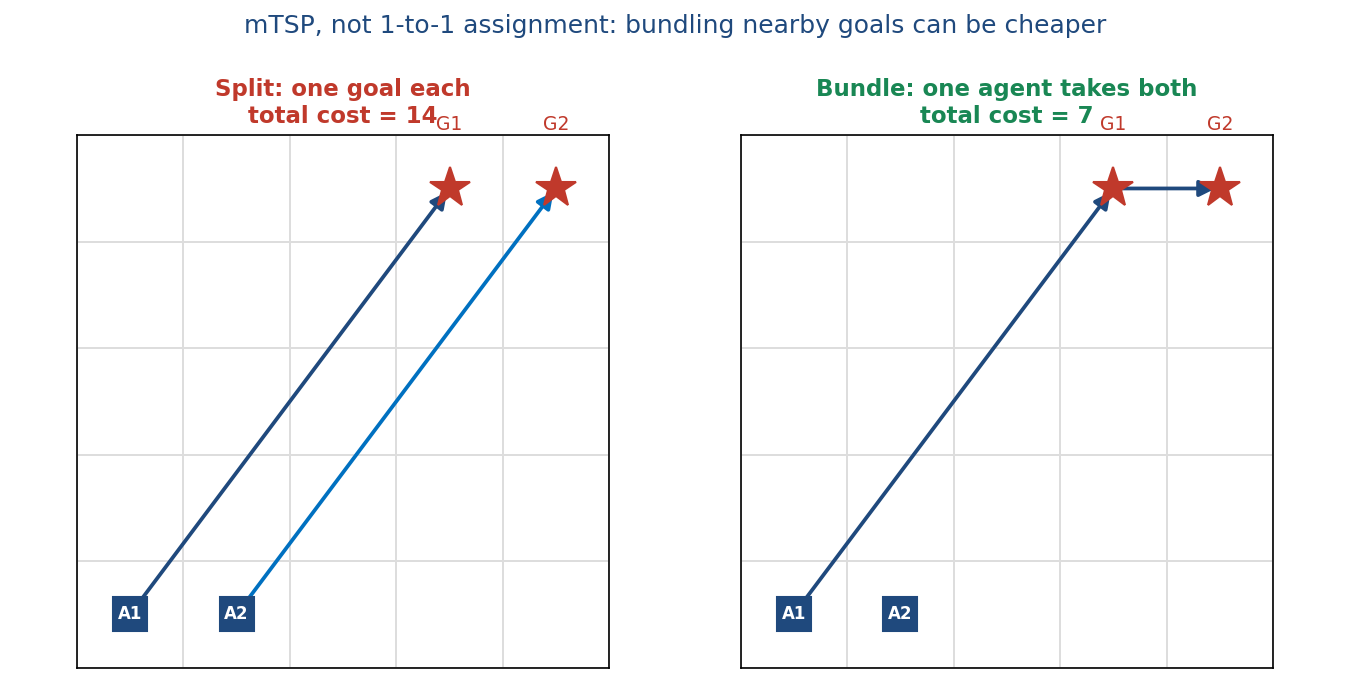
\includegraphics[width=0.58\textwidth]{bundle_vs_split.png}
\caption{Goal allocation is an mTSP, not a balanced assignment. Bundling both goals onto one
agent (cost 7) beats splitting them (cost 14). }
\label{fig:bundle}
\end{figure}

Write $Y \in \{0,1\}^{N \times M}$ for the allocation: one row per agent and one column per goal, so
$Y$ has $N$ rows and $M$ columns, and $Y_{ij}=1$ exactly when agent $i$ visits goal $j$. Reading
down column $j$ answers ``which agent takes this goal'', and that column holds exactly one 1,
because every goal is visited once by one agent. Reading across row $i$ answers ``which goals does
this agent get'', and that row may hold any number of 1s, including none, because an agent is free
to take several goals or sit idle. Columns therefore sum to one while rows are unconstrained.

The same shape runs through the whole model. The input $D$ and the output $P$ are both $N \times M$
with agents on the rows and goals on the columns, so all three matrices line up entry for entry,
while $G$ is $M \times M$ because it relates goals to each other rather than agents to goals. The
model therefore has to produce a column-wise distribution, giving for each goal a distribution over
agents, instead of a doubly-stochastic or permutation-like output. This rules out Sinkhorn-style
balanced-assignment layers, which impose a row constraint the problem does not have.

\subsection{The exact baseline}

RobustMCPF in BasicMAPF mode serves as both ground truth and comparison point. It calls LKH to
solve the underlying TSP, which yields $k$-best allocations along with each agent's visit order,
and then runs CBS to resolve conflicts. We take the cost of the final collision-free plan as the
definitive quality measure. The same solver generates the training labels: every training instance
is solved exactly, and its allocation becomes the supervision target.

\subsection{Related work}

Learning to solve combinatorial problems has a substantial literature. Pointer
Networks~\cite{pointernet} output permutations of their input, reinforcement-learning variants
scaled the idea to routing~\cite{bello}, and attention models became the standard backbone for TSP
and VRP~\cite{kool}; \cite{bengio} surveys the area. Within MAPF, CBS~\cite{cbs} defines the
exact-planning baseline, benchmarks and terminology come from~\cite{stern,sturtevant}, and learned
policies such as PRIMAL~\cite{primal} target path planning, not allocation. Combined target
assignment and planning was formalized by~\cite{ma_koenig}. Closest to our final study is algorithm
selection for MAPF~\cite{kaduri}, which asks the same underlying question of whether
instance-specific specialization beats one general method. We differ from the routing literature in
learning only the allocation and leaving an exact planner downstream, which makes the comparison
end-to-end and unambiguous.

% ═════════════════════════════════════════════════════════════════════════════
\section{Method: The Learned Allocator}
\label{sec:method}
% ═════════════════════════════════════════════════════════════════════════════

\subsection{Overview}

The solver runs LKH followed by CBS. Ours runs a forward pass through the network, then goal-visit
ordering, then CBS (Figure~\ref{fig:pipelines}). Both pipelines plan collision-free paths with the
same CBS implementation. They differ in how the visit order within each agent's goals is obtained:
LKH returns it as part of its tour, whereas our pipeline computes it separately once the allocation
is fixed.

\begin{figure}[htbp]
\centering
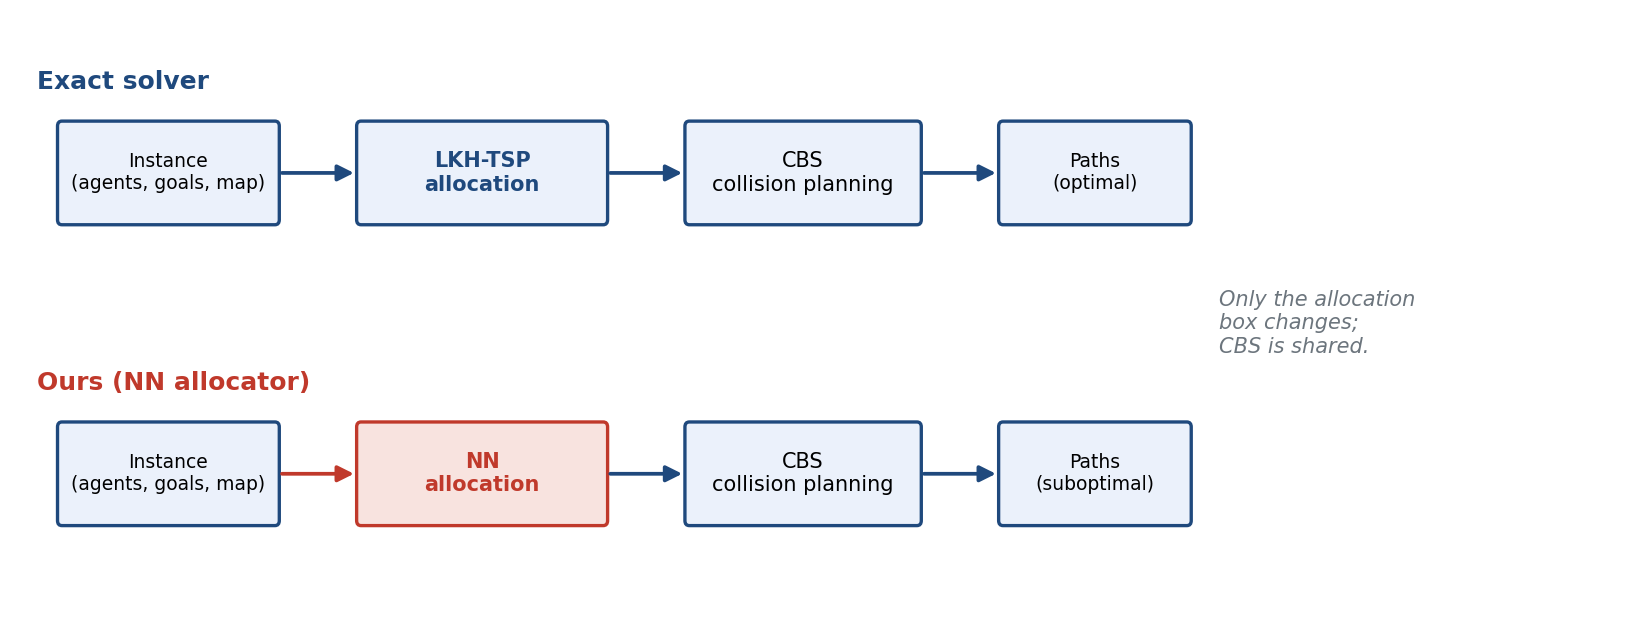
\includegraphics[width=0.86\textwidth]{pipeline_solver_vs_nn.png}
\caption{Only the allocation box changes. CBS is shared, so any difference in execution cost or
wall-time can be attributed to the allocator.}
\label{fig:pipelines}
\end{figure}

\subsection{Input representation}

The network never sees the grid. It sees two matrices of BFS shortest-path distances that respect
walls: $D \in \mathbb{R}^{N \times M}$ from each agent to each goal, and $G \in \mathbb{R}^{M \times
M}$ between goals (Figure~\ref{fig:dg}). Both are divided (normalized) by $(W-1)+(H-1)$, where $W$ and $H$ are the
grid's width and height in cells. This is the longest shortest path on an open grid of that size,
so it puts distances from grids of different sizes on a common scale. Walls can force a detour that
exceeds it, so it is a scale factor and not a strict bound.

Using distances instead of coordinates is a deliberate choice. Tour cost is a function of
distances, and distances abstract away the map, so the representation transfers across grid sizes
and geometries. $D$ tells each agent how far each goal is. $G$ carries the information $D$ cannot
express, which is which goals lie near each other and should therefore be bundled onto one agent.
Section~\ref{sec:design} shows that $G$ is the single most valuable design decision in the project.

\begin{figure}[H]
\centering
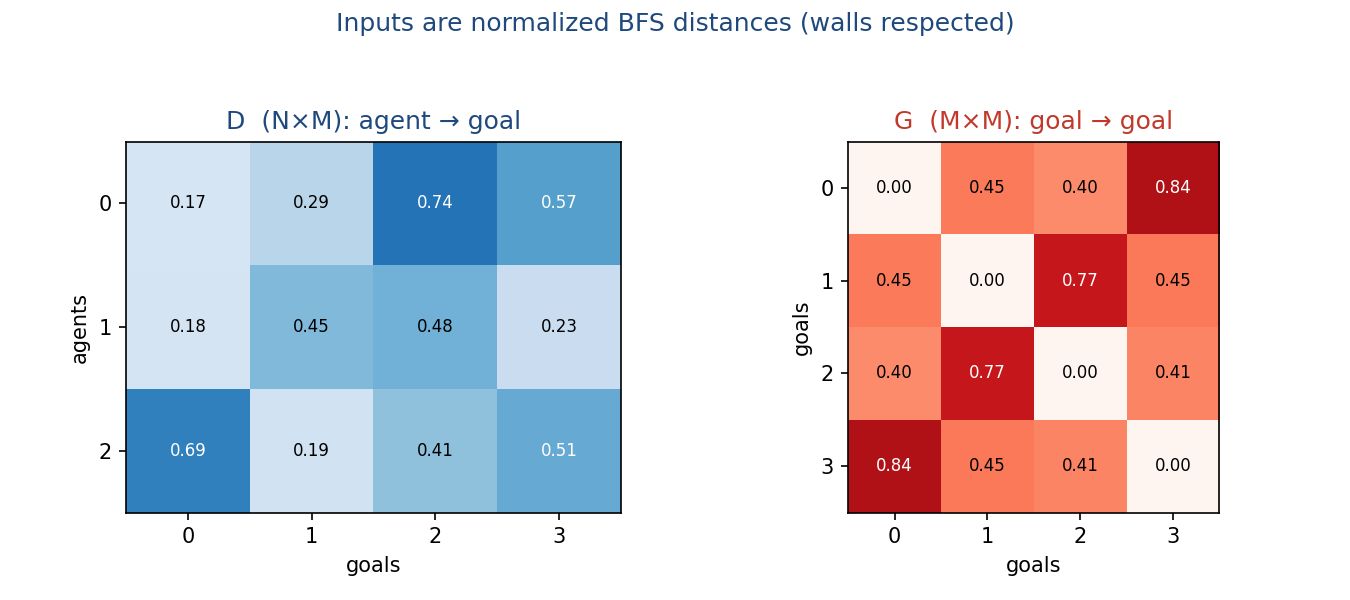
\includegraphics[width=0.54\textwidth]{D_G_matrices.png}
\caption{The two inputs for one instance: agent-to-goal distances $D$ and goal-to-goal distances
$G$, both normalized BFS distances with walls respected.}
\label{fig:dg}
\end{figure}

\subsection{Handling any number of agents and goals}
\label{sec:anynm}

A conventional network fixes its input dimension, which would force one model per $(N,M)$ pair.
Ours does not, and the mechanism is worth setting out in full (Figure~\ref{fig:anynm}).

\textbf{Tokenization.} Each scalar $D_{ij}$ is projected independently to a $d$-dimensional vector
by a shared $\mathrm{Linear}(1 \to d)$, producing an $N \times M$ grid of tokens. Because the
projection is shared, the parameter count does not depend on $N$ or $M$.

\textbf{Goal context.} Goal $j$ has a row of distances to every other goal, $G_{j1}$ through
$G_{jM}$. Each of those numbers is passed through its own shared $\mathrm{Linear}(1 \to d)$, turning
it into a $d$-dimensional vector, and the resulting vectors are then added together elementwise to
give a single $d$-dimensional summary for goal $j$. Embedding before adding matters, because it lets
the network retain more than one property of the distances, and because the sum of any number of
$d$-vectors is still a $d$-vector, $M$ can be anything. That summary is added to each of the $N$
tokens in goal $j$'s column, which are $d$-dimensional as well, so every token concerning goal $j$
also carries information about how that goal sits relative to the rest.

\textbf{Attention.} Each block applies row attention, in which an agent attends over its own goals
and learns how they relate to each other, then column attention, in which a goal attends over the
candidate agents and learns which is best placed to take it, then a feed-forward layer. Blocks are
stacked $L$ deep. Attention operates on variable-length sequences by construction.

\textbf{No positional embeddings.} Agents and goals are unordered sets in an mTSP, so there is no
meaningful ``agent 1''. Leaving out positional embeddings makes the network permutation-equivariant
in both axes and removes the last size-dependent component, which is why the same weights can
process a $2\times2$ instance and a $50\times100$ one.
The architecture therefore places no upper bound on $N$ or $M$. 

\textbf{Output.} A shared $\mathrm{Linear}(d \to 1)$ reduces each token to a single logit, giving an
$N\times M$ logit matrix. A softmax down each column yields $P$, where $P_{ij}$ is the probability
that agent $i$ visits goal $j$ and $\sum_i P_{ij}=1$. This is exactly the structure
Section~2.2 requires. Taking the arg-max of each column decodes the binary allocation.

\textbf{Mixed-size training.} Instances of different shapes cannot be stacked into one rectangular
array, which is what a GPU needs in order to process many at once, so a
\texttt{MixedSizeBatchSampler} builds shape-homogeneous batches. Each batch holds a single $(N,M)$
while consecutive batches differ, which trains one model jointly across many configurations without
padding or masking.

\textbf{A worked example.} Take $N{=}3$ agents, $M{=}4$ goals and embedding width $d{=}128$. Here
$D$ is $3\times4$ and $G$ is $4\times4$. Tokenization turns each of the 12 entries of $D$ into a
128-vector, giving a $3\times4$ grid of tokens. For goal 2, the four numbers $G_{21}$ through
$G_{24}$ each become a 128-vector and are summed into one 128-vector, which is added to all three
tokens in column 2. Row attention then runs over sequences of length 4, once per agent; column
attention runs over sequences of length 3, once per goal. The head reduces every token to a single
number, giving a $3\times4$ logit matrix, and a softmax down each of the four columns gives each
goal a distribution over the three agents. Now change the instance to $N{=}180$ and $M{=}350$: the
token grid becomes $180\times350$, attention runs over sequences of length 350 and 180 instead of 4
and 3, and every weight in the network is the same one used for the $3\times4$ case.

\begin{figure}[htbp]
\centering
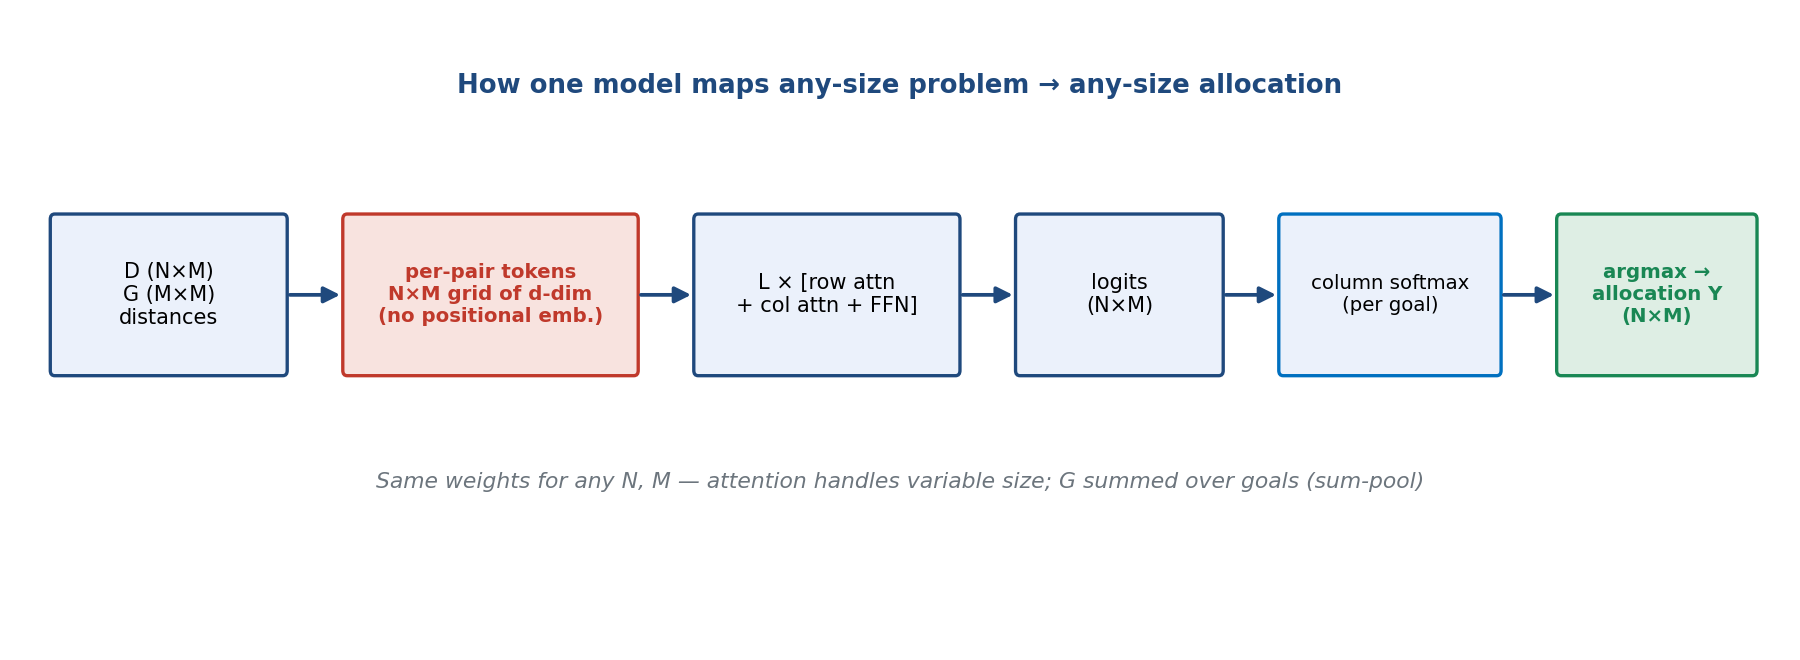
\includegraphics[width=0.96\textwidth]{anyNM_pipeline.png}
\caption{The size-agnostic path from an instance to an allocation. $D$ and $G$ become an $N\times M$
token grid, row/column attention blocks process it, a shared head produces $N\times M$ logits, a
column softmax gives a per-goal distribution over agents, and arg-max decodes the allocation. No
stage depends on the values of $N$ or $M$.}
\label{fig:anynm}
\end{figure}

\subsection{Loss}

Training minimizes
\[
\mathcal{L} = \mathcal{L}_{\mathrm{CE}} + \lambda\,\mathcal{L}_{\mathrm{MinSum}},
\qquad
\mathcal{L}_{\mathrm{CE}} = -\tfrac{1}{M}\textstyle\sum_{j}\sum_{i} Y_{ij}\log P_{ij},
\qquad
\mathcal{L}_{\mathrm{MinSum}} = \tfrac{1}{M}\textstyle\sum_{i,j} P_{ij} D_{ij},
\]
with $\lambda = 0.1$. The cross-entropy term is per-goal imitation of the solver and does most of
the work. The min-sum term is a mild geometric regularizer that penalizes assigning distant goals
and prevents degenerate near-uniform predictions early in training. It is only a first-hop proxy,
with no tour chaining and no collision term, so the true mTSP objective reaches training solely
through the labels $Y$.

Training directly on the solver's true post-allocation cost would target the objective we actually
measure, but it is impractical at these scales. The cost is only defined once a discrete allocation
has been decoded from $P$ and CBS has planned around the conflicts, so as a function of the
network's output it is a step function: small changes in $P$ leave it unchanged until an arg-max
flips, and then it jumps. Gradient descent has nothing to follow. Estimators that do not need a
gradient, policy-gradient methods among them, exist and would apply, but they need many cost
evaluations per update, and every evaluation is a CBS solve costing seconds to a minute at the
scales of Section~\ref{sec:final}. Labels, by contrast, are generated once and then reused across
all 50 epochs. Imitating the solver's allocation recovers most of the signal for a small fraction
of that compute, which is why the collision-aware alternatives are left to future work.

\subsection{Data generation and deployment}
\label{sec:deploy}

Each sample is produced by placing agents and goals on a map, computing $D$ and $G$ by BFS, and
calling the solver for the optimal $Y$. Instances with unreachable goals are rejected, as are those
that exceed a CBS node budget of 50k expansions. That second filter addresses a failure mode found
at high wall density, where an instance passes the reachability check but CBS escalates constraints
without ever terminating.

At deployment the arg-max allocation is decoded, each agent's visit order is fixed, and CBS plans
the paths. Ordering is done by exhaustive enumeration: for an agent holding $k$ goals we evaluate
all $k!$ orderings and keep the cheapest, which is optimal by construction. Beyond eight goals per
agent the enumeration becomes impractical, so we fall back to nearest-neighbor construction followed
by 2-opt improvement. When an allocation admits no
collision-free plan, the next candidate in a probability-ranked chain is tried, taken best-first
over the joint probability $\prod_j P_{a_j,j}$ up to $k=3$. This is the learned counterpart of the
solver's $k$-best escape.

% ═════════════════════════════════════════════════════════════════════════════
\section{Experimental Setup and Metrics}
\label{sec:setup}
% ═════════════════════════════════════════════════════════════════════════════

Experiments run on procedurally generated grids and on the four $32\times32$ benchmark maps that
RobustMCPF itself uses (Figure~\ref{fig:maps}). Only \texttt{maze} and \texttt{room} have genuine
corridor and room structure, while \texttt{empty} and \texttt{random} are unstructured. That
distinction drives several of the results below.

\begin{figure}[htbp]
\centering
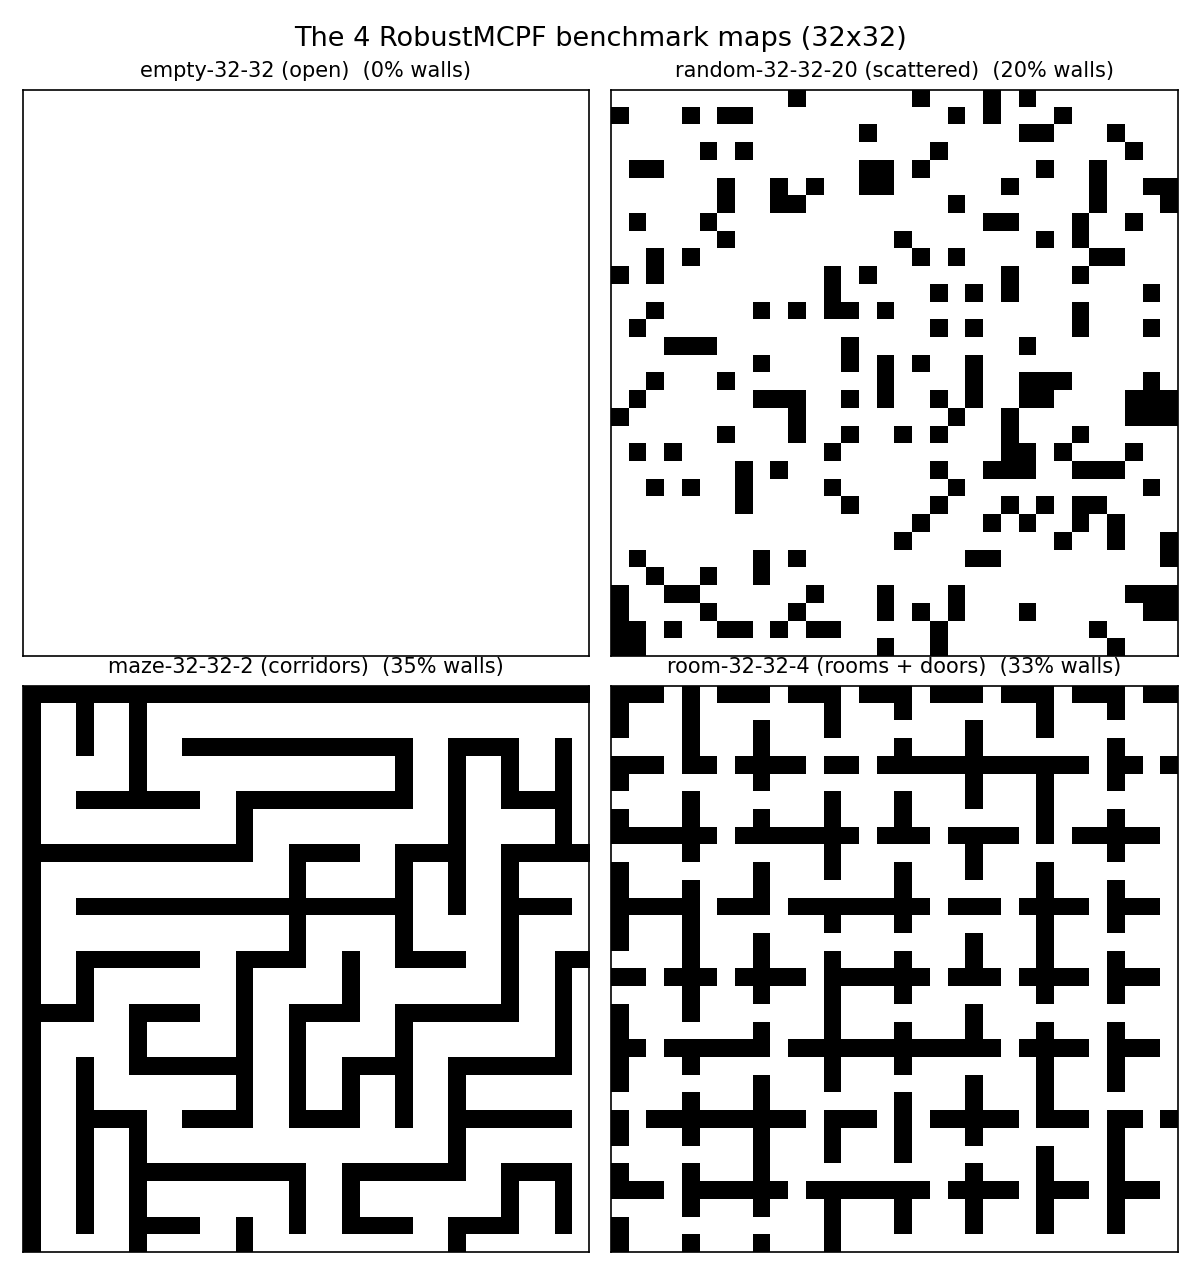
\includegraphics[width=0.46\textwidth]{maps_panel.png}
\caption{The four $32\times32$ benchmark maps: \texttt{empty}, \texttt{random-32-32-20},
\texttt{maze-32-32-2} and \texttt{room-32-32-4}. Only the last two are structured.}
\label{fig:maps}
\end{figure}

\textbf{Allocation-quality metrics} compare predicted and ground-truth allocations directly, with
no planning involved. Per-goal accuracy is the fraction of goals routed to the solver's chosen
agent. It is a lenient measure, since one wrong goal out of $M$ still scores $(M{-}1)/M$.
Full-assignment accuracy is the all-or-nothing indicator that every column matches, and it
empirically tracks (per-goal accuracy)$^{M}$. A proxy cost ratio compares only the first-hop BFS
cost of the two allocations. Because it ignores tour chaining and collisions, values below $1.0$
reflect the metric's mismatch with the true objective and not the network beating the solver.

\textbf{Execution-cost metrics} run both pipelines end to end, where a plan's cost is the total
collision-free path length in grid steps that CBS returns. Cost ratio is the per-instance
$c_{\mathrm{nn}}/c_{\mathrm{sol}}$ averaged over instances, so $1.0$ means the network matched the
exact solver. Exact match is the fraction of instances whose two integer costs are identical, and
it runs far higher than full-assignment accuracy because many distinct allocations are
cost-equivalent ties. 

\textbf{Diff} is the mean gap in grid steps, \textbf{speedup} is the ratio of mean
single-instance wall-times on the same node, and the \textbf{infeasible} and \textbf{fallback} counters report how often the candidate chain was needed. These are the numbers that matter, because they measure the
plan an agent would actually execute.

% ═════════════════════════════════════════════════════════════════════════════
\section{Design Study: What Shaped the System}
\label{sec:design}
% ═════════════════════════════════════════════════════════════════════════════

Fifteen experiments preceded the final system. Instead of recounting them chronologically, we
report the five findings that determined the design, each of which fixes one property described in
Section~\ref{sec:method}. Table~\ref{tab:decisions} collects the supporting numbers. Throughout this
section $N$ is the number of agents and $M$ the number of goals, and differences in accuracy are
quoted in percentage points: a model scoring 0.789 against one scoring 0.772 is ahead by 1.7 points.

\textbf{D1. Attention wins, and increasingly so with scale.} Against an MLP and a DeepSets encoder
on identical data, the row/column transformer led on every metric, and its margin over the MLP grew
from $1.7$ points of full-assignment accuracy at $N{=}2$ to $6.7$ points at $N{=}5$. Cross-goal
interdependence is what widens as problems grow, and attention is what captures it. This fixes the
backbone.

\textbf{D2. Representation dominates everything else.} Adding $G$ lifted full-assignment accuracy
by 14 to 18 points at every agent count. For comparison, doubling the training set from 10k to 20k
samples bought $0.4$ points, and every capacity increase we tried bought at most $1.4$, with the
largest configuration diverging outright. $D$ on its own cannot express the fact that two goals are
adjacent and should be bundled. $G$ supplies precisely that, and it is worth more than architecture,
data and capacity put together: about four times as much at $N{=}2$ and roughly twice as much at
$N{=}5$. This fixes the input.

\textbf{D3. One size-agnostic model beats a family of fixed-size models.} A universal model trained
jointly across fifteen $(N,M)$ configurations matched or beat the fixed-size models on all but
the easiest configuration, gaining $2.4$ to $3.5$ points. It also transferred upward. Evaluated on
$N{=}5$, which it had never seen in training, it beat the model built specifically for $N{=}5$ by
$3.5$ points. Cross-configuration training acts as a regularizer and pushes the model toward the
allocation principle instead of size-specific patterns. This justifies the universal architecture.

\textbf{D4. Allocation accuracy is the wrong yardstick.} Measured end to end, the fraction of
instances whose plan costs exactly what the solver's costs (64--97\%) far exceeds the fraction on
which the same allocation is chosen (44--91\%). Many disagreements are ties, with two agents
equidistant from a goal and either choice equally good, so a model judged on allocation accuracy
alone looks considerably worse than it performs. This is why every headline number in this report
is an execution cost.

\textbf{D5. Geometry transfers, scale does not.} A model trained only on small random grids and
evaluated zero-shot on the four real maps at small $N,M$ reached a cost ratio of $1.019$, meaning no
meaningful degradation. Structured maps even proved easier than open ones, because walls remove the
ties that an open grid leaves to chance. Pushed to large $N,M$, the same model collapsed to $1.246$
against a map-trained model's $1.048$, with a revealing signature: at $M{=}30$, adding agents hurt
the model trained on $N\le5$ while helping the in-range model (Figure~\ref{fig:designfigs}b).
Separately, training on cheap random grids matched training on the real maps everywhere except the
maze, where random obstacles never reproduce corridor structure. This is why the final models are
retrained at the target scale and on the target maps, and it is the direct motivation for
Section~\ref{sec:final}.

\begin{table}[htbp]
\centering
\caption{Design decisions and the evidence behind them. Effects are on full-assignment accuracy
(D1--D3) or execution-cost ratio (D4--D5).}
\small
\begin{tabularx}{\textwidth}{llX}
\toprule
\textbf{Decision} & \textbf{Effect} & \textbf{Evidence} \\
\midrule
Transformer backbone            & $+1.7 \to +6.7$ pt   & vs.\ MLP, margin growing over $N{=}2\ldots5$ \\
\textbf{Add goal-goal distances $G$} & $\mathbf{+14.2 \to +18.0}$ \textbf{pt} & with vs.\ without $G$, all agent counts \\
More data (10k $\to$ 20k)       & $+0.4$ pt            & gains already flattening at 20k \\
More capacity (to h256/L6)      & $\le +1.4$ pt        & largest configuration diverges at lr $10^{-3}$ \\
Size-agnostic universal model   & $+2.4 \to +3.5$ pt   & vs.\ fixed-size models; $+3.5$ pt zero-shot at $N{=}5$ \\
Judge by CBS execution cost     & 64--97\% vs.\ 44--91\% & exact-cost match vs.\ exact-allocation match \\
Train on the target map family  & $1.048$ vs.\ $1.075$ & fixed-map vs.\ random; the gap is entirely the maze ($1.029$ vs.\ $1.127$) \\
Retrain at the target scale     & $1.048$ vs.\ $1.246$ & map-trained vs.\ small-scale model at large $N,M$ \\
Smaller network in-distribution & $1.048$ vs.\ $1.052$ & h128/L6 vs.\ h256/L8; $2.5\times$ the parameters bought nothing \\
\bottomrule
\end{tabularx}
\label{tab:decisions}
\end{table}

\begin{figure}[htbp]
\centering
\begin{minipage}[b]{0.475\textwidth}
  \centering
  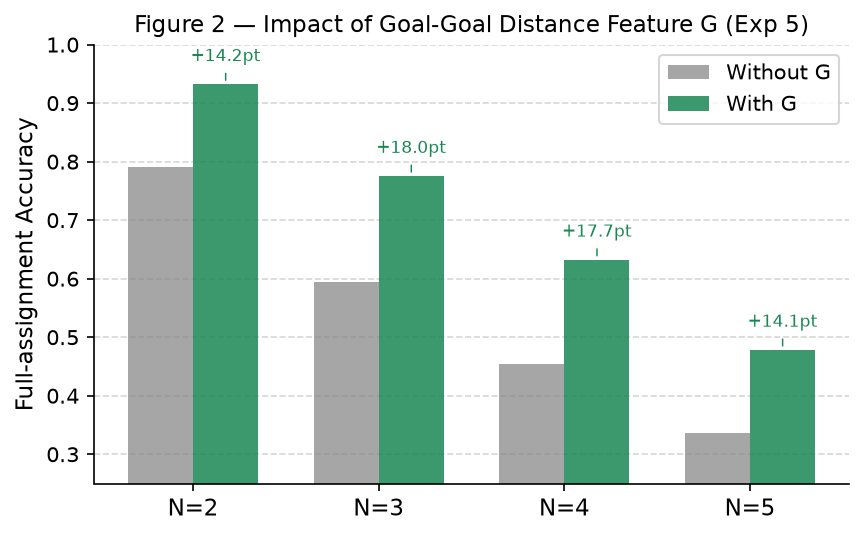
\includegraphics[width=\textwidth]{fig2_ablation.png}\\[1pt]
  {\small (a) the $G$ ablation}
\end{minipage}\hfill
\begin{minipage}[b]{0.475\textwidth}
  \centering
  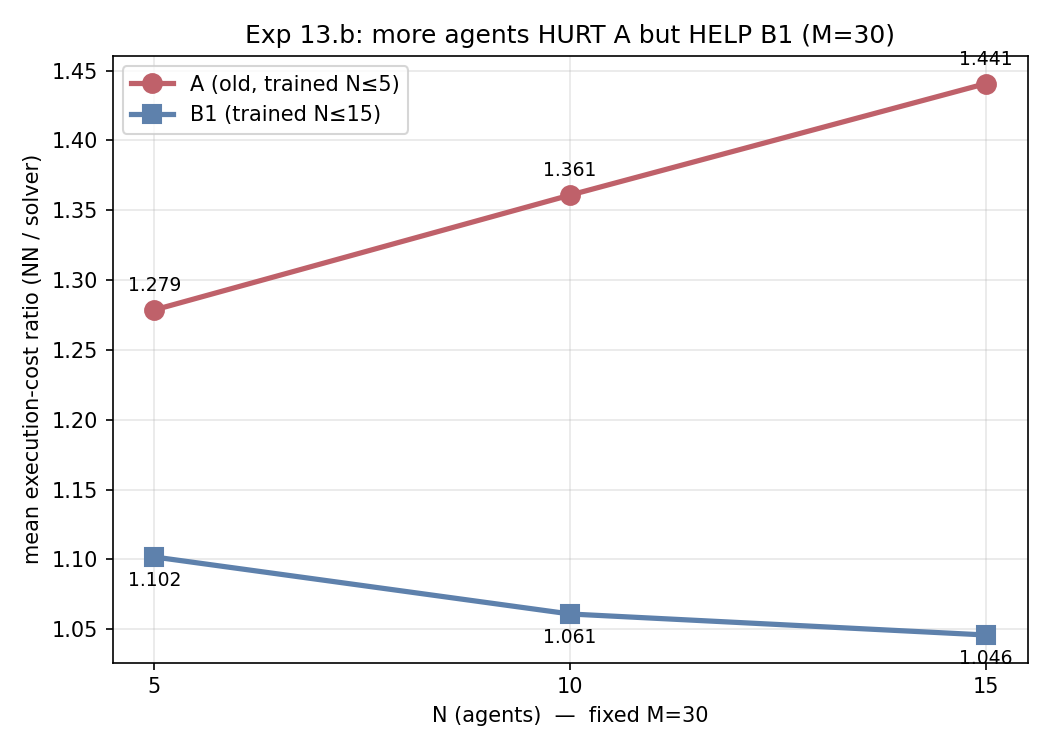
\includegraphics[width=\textwidth]{fig2_N_divergence_m30.png}\\[1pt]
  {\small (b) the scale-transfer scissors}
\end{minipage}
\caption{The two findings that set up the final study. \textbf{(a)} Goal-to-goal distances lift
full-assignment accuracy by 14 to 18 points at every agent count, the dominant design decision (D2).
\textbf{(b)} At $M{=}30$, adding agents hurts the small-scale-trained model but helps the map-trained
one, so generalization fails across problem scale, not across map geometry (D5).}
\label{fig:designfigs}
\end{figure}

\begin{findingbox}{Why this leads to the final study}
D5 showed that a model has to be trained on structured geometry in order to handle it, since the
entire advantage of map-based training over random-grid training came from the maze. If
geometry-specific structure matters that much, the natural next question is whether a dedicated
model per map outperforms one generalist serving all four. That is what Section~\ref{sec:final}
tests.
\end{findingbox}

% ═════════════════════════════════════════════════════════════════════════════
\section{Final Study: Scale Limits and Specialists versus a Generalist}
\label{sec:final}
% ═════════════════════════════════════════════════════════════════════════════

\subsection{Research questions}

\begin{enumerate}[label=\textbf{RQ\arabic*.}]
  \item How far can $N$ and $M$ grow before the exact solver becomes impractical, on the order of a
        minute per instance, and what does that imply for what can be labeled and measured?
  \item For each model role, which training distribution works better: many instances at regular
        size, or fewer instances at large size?
  \item Do per-map specialists outperform a single generalist, in quality and in wall-time, by
        enough to justify routing an instance to a map-specific model?
\end{enumerate}

\subsection{Design}

\textbf{The scale wall.} We sweep $N$ and $M$ on each map until the solver's mean wall-time
approaches 60 seconds (Figure~\ref{fig:scalewall}, interpreted under RQ1 below). This wall is what
bounds the study: every training label still needs an exact solve, so it caps what a large-instance
dataset can contain, and it caps how far a cost-ratio comparison can even be evaluated, since past
it there is no solver baseline left to divide by.

\textbf{Two training regimes.} We compare two training datasets, named for what separates them. The
\textbf{large dataset} covers $N\in\{60,120,180\}$, $M\in\{100,225,350\}$, with 3000 train / 500 val
/ 500 test instances per configuration, labeled at a per-instance solver time that on the hardest
cells approaches the practical one-minute ceiling above. The \textbf{regular dataset} covers
$N\in\{30,55,80\}$, $M\in\{50,100,150\}$, with 20000/2000/2000 instances per configuration, labeled
in roughly ten seconds per instance, which buys $6\times$ more samples per configuration. Five
roles, one generalist trained on all four maps and four specialists trained on \texttt{empty},
\texttt{random}, \texttt{maze} and \texttt{room} respectively, are each trained once on each dataset:
five \textbf{large-dataset models} (Table~\ref{tab:modelinv}) and five \textbf{regular-dataset
models} (Table~\ref{tab:modelinvB}). Ten models in total, all h128/L6.

\textbf{Why only the smaller architecture.} We fix the network to h128/L6 because it beat the larger
h256/L8 in-distribution on every aggregate metric, with a $1.048$ versus $1.052$ execution-cost
ratio and $0.433$ versus $0.402$ exact match, while running roughly 20\% faster. The extra
$2.5\times$ in parameters bought no accuracy, and the larger model reached its validation optimum
early and then overfitted. The ranking does reverse far out of distribution, where the larger model
extrapolates better, but the large dataset places the large-instance regime inside the training distribution
by construction, so the in-distribution verdict is the applicable one.

\textbf{Protocol.} All models see identical instances for a given (map, $N$, $M$) cell, which allows
paired comparison. The dataset choice for RQ2 is made on validation data, and the
specialist-versus-generalist comparison for RQ3 is reported on held-out test data, so the selection
step cannot inflate the final result. The generalist is scored per map and not pooled. Without
that, a uniformly mediocre generalist would be indistinguishable from one that is strong on three
maps and weak on the fourth.

\begin{table}[htbp]
\centering
\caption{Model inventory, large-dataset leg (five roles).}
\small
\begin{tabularx}{\textwidth}{llXcccc}
\toprule
Model & Role & Train map(s) & $N$ range & $M$ range & Epochs & Batch \\
\midrule
\texttt{tierA\_joint}   & generalist & all four & 60--180 & 100--350 & 50 & 4 \\
\texttt{tierA\_empty}   & specialist & empty & 60--180 & 100--350 & 50 & 4 \\
\texttt{tierA\_random}  & specialist & random & 60--180 & 100--350 & 50 & 4 \\
\texttt{tierA\_maze}    & specialist & maze & 60--180 & 100--350 & 50 & 4 \\
\texttt{tierA\_room}    & specialist & room & 60--180 & 100--350 & 50 & 4 \\
\bottomrule
\end{tabularx}
\label{tab:modelinv}
\end{table}

\begin{table}[htbp]
\centering
\caption{Model inventory, regular-dataset leg (five roles).}
\small
\begin{tabularx}{\textwidth}{llXcccc}
\toprule
Model & Role & Train map(s) & $N$ range & $M$ range & Epochs & Batch \\
\midrule
\texttt{tierB\_joint}   & generalist & all four & 30--80 & 50--150 & 50 & 32 \\
\texttt{tierB\_empty}   & specialist & empty & 30--80 & 50--150 & 50 & 32 \\
\texttt{tierB\_random}  & specialist & random & 30--80 & 50--150 & 50 & 32 \\
\texttt{tierB\_maze}    & specialist & maze & 30--80 & 50--150 & 50 & 32 \\
\texttt{tierB\_room}    & specialist & room & 30--80 & 50--150 & 50 & 32 \\
\bottomrule
\end{tabularx}
\label{tab:modelinvB}

\smallskip
\small\noindent Both tiers share the h128/L6 universal architecture, about 1.19M parameters (the
same as Exp 12's h128/L6), lr $5\times10^{-4}$ and gradient clipping 1.0; seed 0 is the one
evaluated throughout. The large-dataset leg trained 3 seeds per role (0--2); the regular-dataset leg trained 2 (0--1, cut from a
planned 3 partway through to let all four per-map configs run in parallel under the cluster's
per-user GPU quota). The large-dataset batch size (4) is far smaller than the regular-dataset one (32) because its
instances are larger ($N,M$ up to $180\times350$) and hit GPU memory limits sooner. Best
validation loss, best epoch and training wall-time are blank for the large-dataset models (only evaluation CSVs
were pulled, not per-epoch logs) and partly blank for the regular-dataset models (available for the four specialists,
not the joint run, whose training history spans several resubmissions and isn't attributable to
one run). Full columns, including what is and is not populated per model, in
\texttt{report/data/exp16/model\_inventory.csv}.
\end{table}

\subsection{Results}

\begin{figure}[htbp]
\centering
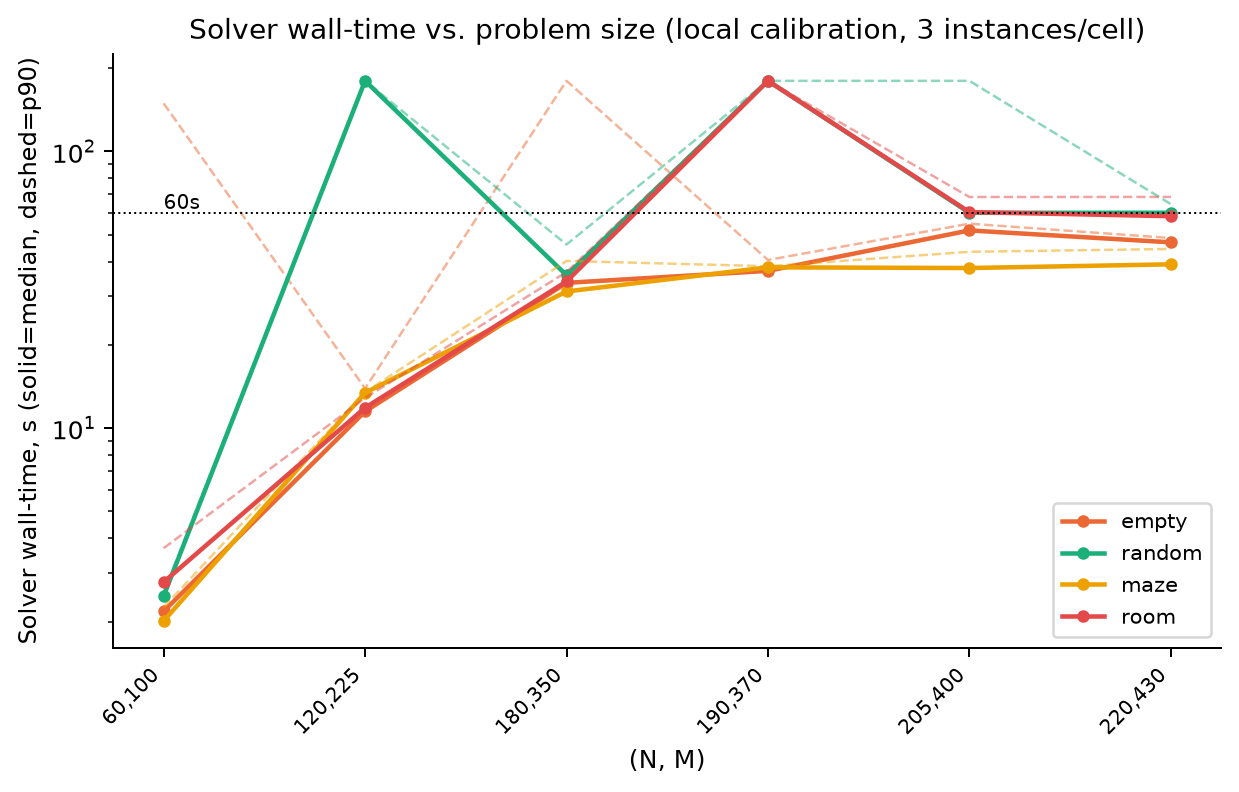
\includegraphics[width=0.72\textwidth]{fig_solver_scale_wall.png}
\caption{Solver wall-time against problem size (local calibration, 3 instances/cell, 180\,s
safety cap). Solid: median. Dashed: p90. The two diverge sharply on \texttt{random} and
\texttt{room}, where a minority of instances are far slower than the typical one.}
\label{fig:scalewall}
\end{figure}

Figure~\ref{fig:scalewall} does not show a clean wall. Median time grows roughly with $(N,M)$ on
\texttt{empty} and \texttt{maze}, 2\,s to 52\,s across the swept range, but on \texttt{random} and
\texttt{room} a minority of individual instances are far slower than the median regardless of
size: at $N{=}120,M{=}225$ on \texttt{random}, 2 of 3 instances hit the 180\,s safety cap while the
median at the next point tested, $N{=}180,M{=}350$, drops back to 36\,s. Because the sweep moves
$N$ and $M$ together rather than independently, we cannot attribute this to one or the other. What
it does show is that a single pathological instance, not the typical one, is what threatens a
fixed compute budget. The \textbf{labeling ceiling} is therefore map-dependent and probabilistic
rather than a fixed $(N,M)$: \texttt{maze} stayed at 0\% timeouts everywhere tested, \texttt{empty}
hit one 33\% cell, and \texttt{random} and \texttt{room} hit 33--67\% timeout rates at some cells
and 0\% at larger ones, which is exactly the profile that motivated the large dataset's
500-sample-per-config size and 600\,s per-instance timeout. The \textbf{evaluation ceiling} is at least $N{=}220,M{=}430$: every
map solved all three instances there, none hit the timeout. We did not observe a size \textbf{beyond}
which the solver stops returning altogether within this sweep, only rising unpredictability, so
that third ceiling is not yet reached at 220$\times$430.

Figure~\ref{fig:stage1crossover} answers RQ2 by evaluating each role's the large dataset and the regular dataset
checkpoints on a common pair of grids spanning both regimes, so every checkpoint is scored both at
home and away. The left panel is the regular dataset's native grid (small, $N\in\{30,55,80\}$,
$M\in\{50,100,150\}$): the regular dataset is interpolating inside its training range there, while the large dataset
is extrapolating downward, to sizes well below anything it ever trained on. The right panel is
the large dataset's native grid (large, $N\in\{60,120,180\}$, $M\in\{100,225,350\}$): the roles reverse,
the large dataset is at home and the regular dataset is extrapolating upward, to sizes beyond anything it ever
trained on.

\begin{figure}[htbp]
\centering
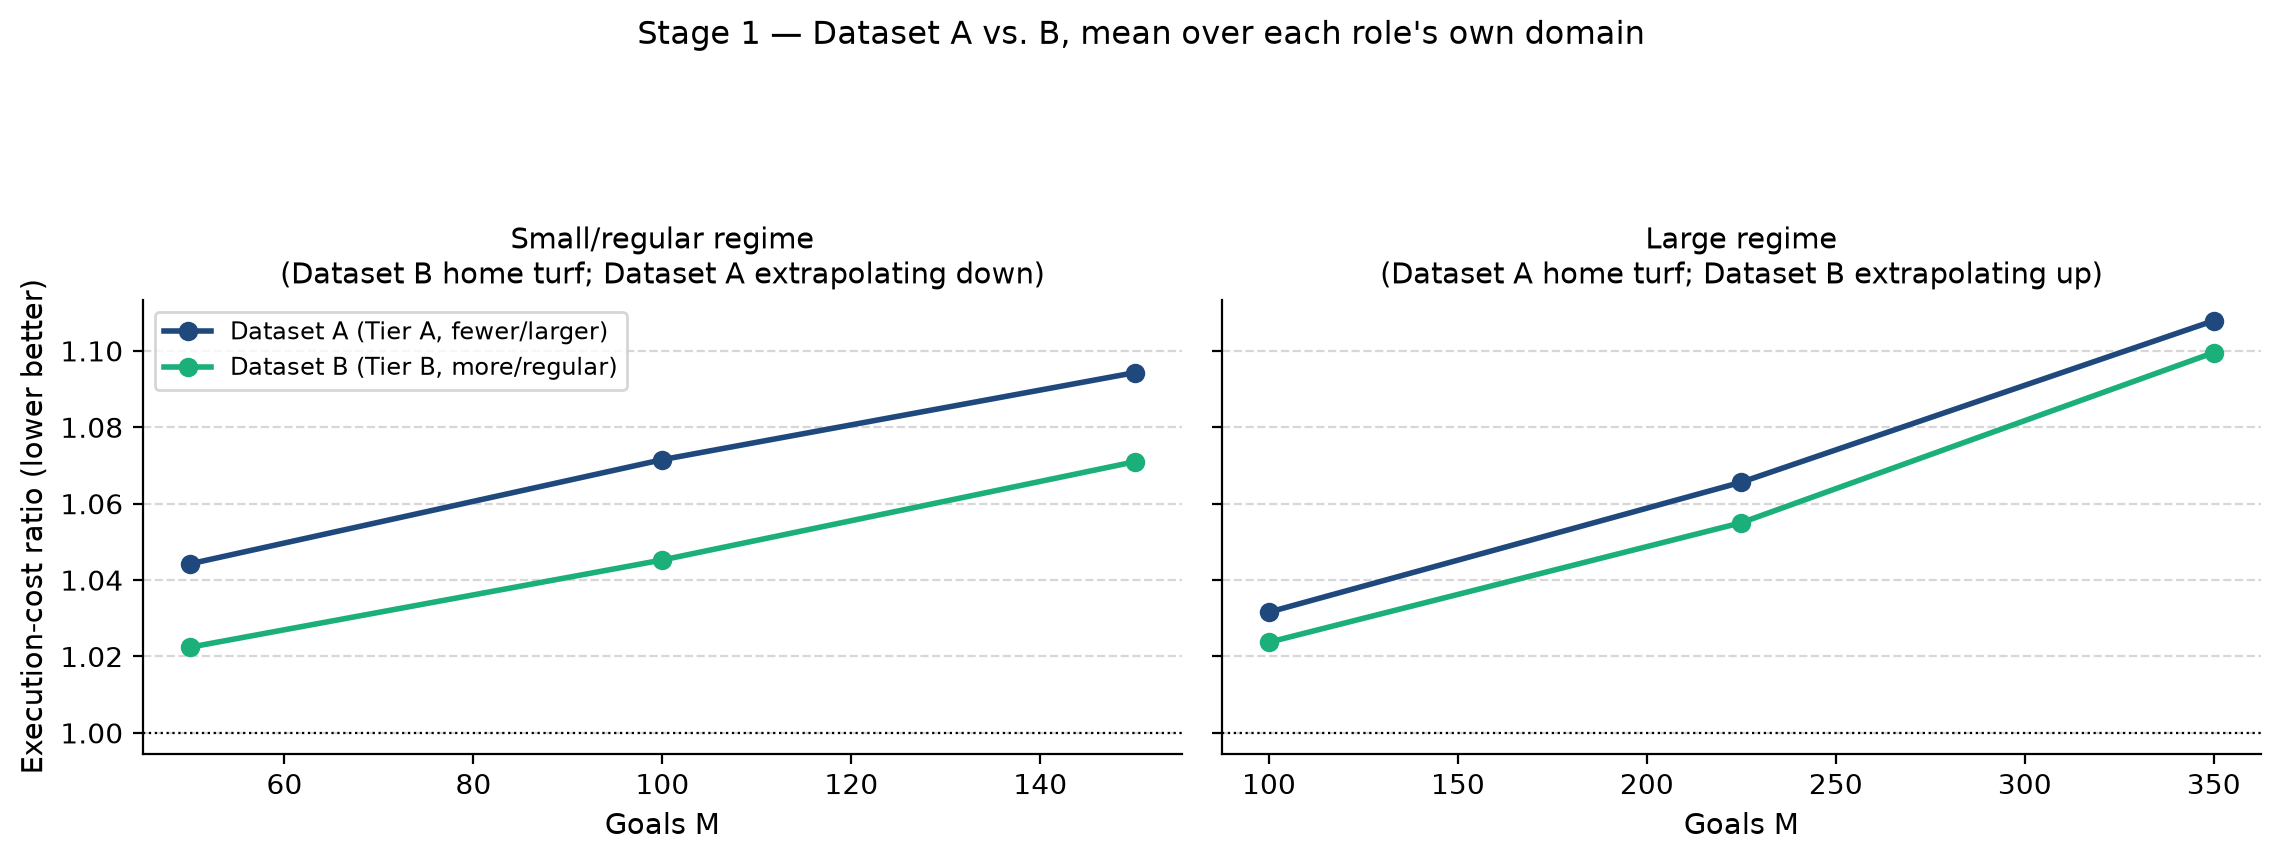
\includegraphics[width=0.85\textwidth]{fig_stage1_crossover.png}
\caption{large vs.\ regular dataset, mean cost ratio over each role's own domain, on both regimes. Solid
lines never cross: the regular dataset (green) sits below the large dataset (navy) at every point in both panels,
whether the regular dataset is interpolating at home (left) or extrapolating up (right).}
\label{fig:stage1crossover}
\end{figure}

% Auto-generated by gen_exp16_stage1.py. Do not edit by hand.
\begin{table}[htbp]
\centering
\caption{Stage 1: dataset A vs.\ B, mean cost ratio over each role's own domain (own map for a specialist, all 4 maps for the generalist), unioned across both grids. Winner is the lower (better) mean.}
\small
\begin{tabularx}{\textwidth}{lXXXl}
\toprule
Role & Dataset A ratio & Dataset B ratio & Margin & Winner \\
\midrule
generalist & 1.055 & 1.070 & 0.015 & A \\
empty & 1.048 & 1.075 & 0.027 & A \\
random & 1.053 & 1.067 & 0.014 & A \\
maze & 1.045 & 1.056 & 0.011 & A \\
room & 1.053 & 1.069 & 0.016 & A \\
\bottomrule
\end{tabularx}
\label{tab:stage1winners}
\end{table}


Table~\ref{tab:stage1winners} confirms it numerically: no crossover for any role. the regular dataset wins
on both its own small grid and on the large dataset's large grid, for all five roles, everywhere it was
tested — including the right panel, where the regular dataset is the one extrapolating and the large dataset is on
native ground. The margin ranges from $0.011$ on \texttt{maze} to $0.027$ on \texttt{empty}, and
the two curves rise together with $M$ rather than swapping order, so the gap is consistent rather
than regime-dependent. This contradicts the RQ2 hypothesis, which expected each dataset to win in
its own regime. The likely explanation is sample count: the regular dataset supplies $6\times$ more
instances per configuration (20k/2k/2k against 3k/500/500), and that advantage evidently
outweighs training directly at the target scale, even when the large dataset is evaluated on its own home
turf. For a fixed labeling budget the result favors many regular-size instances over fewer large
ones: the regular dataset's checkpoints extrapolate to the large regime better than the large dataset's checkpoints
perform natively there, at a fraction of the per-instance solver cost needed to generate the
labels in the first place.

\begin{table}[htbp]
\centering
\caption{Joint (generalist) versus the native specialist, large-dataset leg, own
$N,M$ grid. Speedup is mean solver wall-time divided by mean NN pipeline wall-time, same node.
$n$ is the total instances evaluated, summed across the model's 9 $(N,M)$ cells
(joint\,/\,specialist), out of a nominal 900 ($9\times100$); shortfalls come from whole eval
cells still missing on the cluster (Table~\ref{tab:fullconfig} in the appendix has the per-cell
breakdown), not from filtered outliers.}
\small
\begin{tabularx}{\textwidth}{lXXXXXXc}
\toprule
& \multicolumn{3}{c}{Joint} & \multicolumn{3}{c}{Specialist} & \\
Map & Ratio & Exact & Speedup & Ratio & Exact & Speedup & $n$ \\
\midrule
empty  & 1.071 & 3.6\% & 9.1$\times$  & 1.072 & 2.9\% & 16.5$\times$ & 800/897 \\
random & 1.074 & 3.6\% & 8.8$\times$  & 1.067 & 3.1\% & 17.1$\times$ & 893/887 \\
maze   & 1.057 & 4.0\% & 12.1$\times$ & 1.057 & 3.0\% & 13.2$\times$ & 899/898 \\
room   & 1.069 & 3.9\% & 10.7$\times$ & 1.066 & 3.8\% & 9.2$\times$  & 786/789 \\
\bottomrule
\end{tabularx}
\label{tab:stage2diag}
\end{table}

\begin{figure}[htbp]
\centering
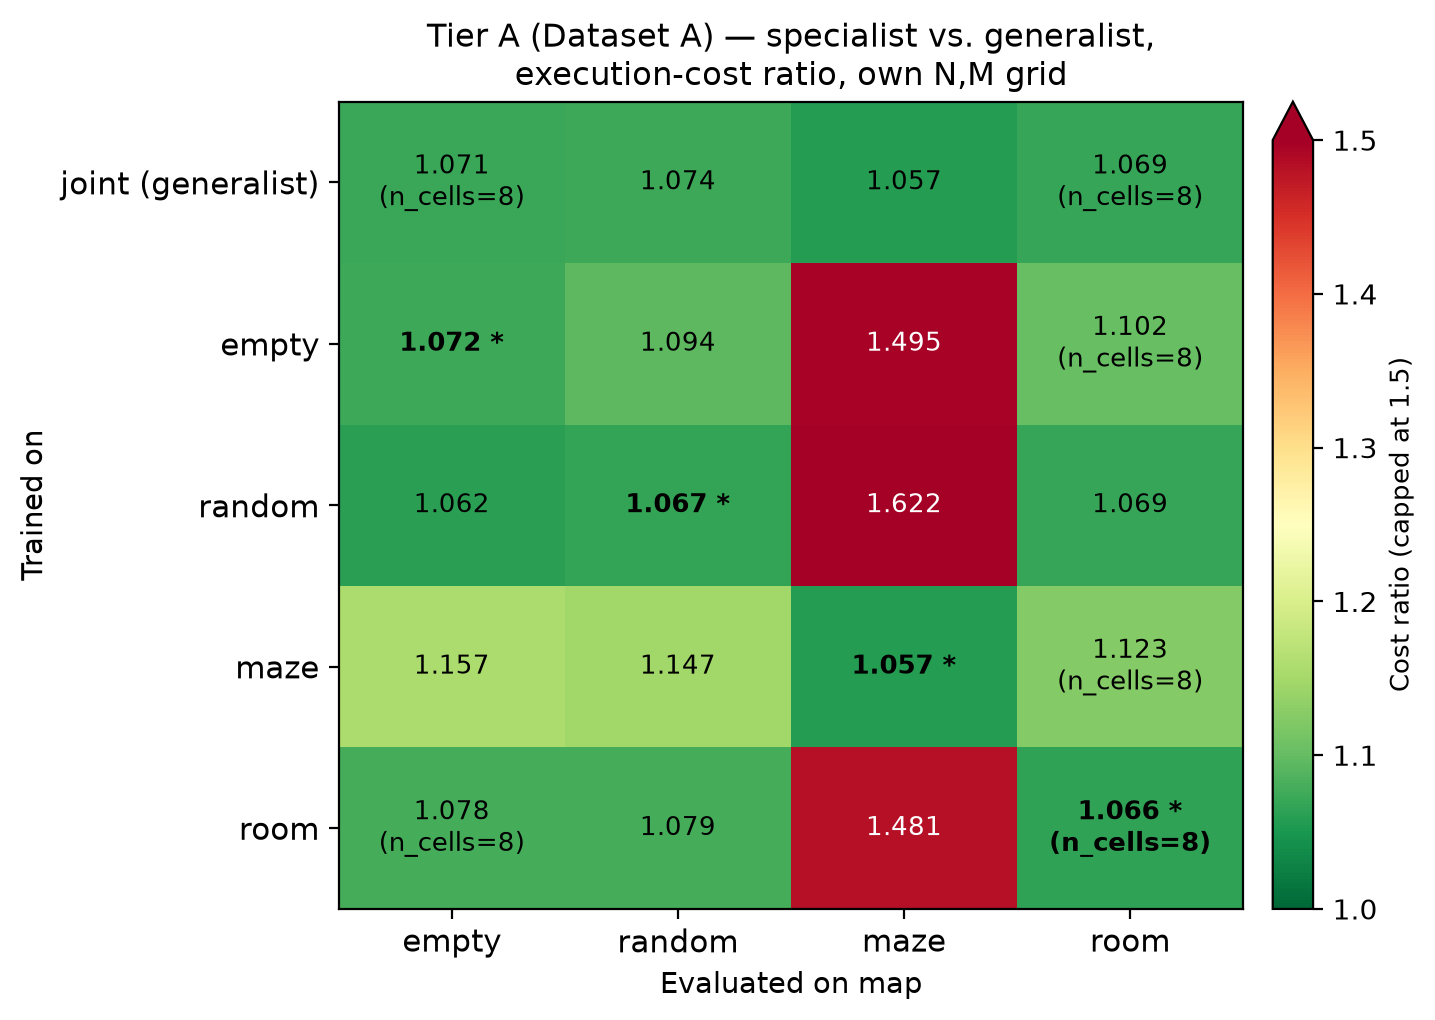
\includegraphics[width=0.62\textwidth]{fig_tierA_5x4_heatmap.png}
\caption{Full $5\times4$ matrix, large-dataset leg: every model (rows) on every map
(columns), execution-cost ratio, own $N,M$ grid. Asterisked cells are a specialist on its own
map. A heatmap is used in place of grouped bars to keep all 20 cells, diagonal and off-diagonal,
legible in one figure.}
\label{fig:tierA54}
\end{figure}

Table~\ref{tab:stage2diag} compares the joint model against each map's native specialist. The two
are close everywhere. The largest gap is 0.007 on random, 1.074 for joint against 1.067 for the
specialist, and maze ties to within 0.001. Neither model dominates the other on cost. The
specialist is faster on three of the four maps, up to 17.1$\times$ on random against 8.8$\times$
for joint, but joint is faster on room. Exact match falls to single digits everywhere, 2.9\% to
4.0\%, well below the 44--91\% range reported at smaller scale in Section~\ref{sec:design}. Ties
in optimal cost become rare as $N$ and $M$ grow, so cost ratio is what still discriminates between
models at this size.

Figure~\ref{fig:tierA54} shows the full $5\times4$ matrix. The diagonal and the joint row sit in a
narrow band, 1.057 to 1.074. The off-diagonal does not. Misrouting an instance costs little on
three of the four maps, empty, random and room all stay under 1.16 when sent to each other's
specialist, but is expensive on maze, where every non-maze specialist reaches 1.48 to 1.62, a 39 to
52\% cost penalty over its own in-distribution number. The effect is not only allocation quality.
Misrouted-to-maze cells also carry far more fallback replanning, mean NN pipeline time 7.2 to
15.2\,s against 2.0 to 2.8\,s in distribution, so a wrong specialist on maze is both a worse plan
and a slower one to produce. This matches the maze-specific transfer gap behind D5: what fails to
transfer across map geometry is maze's corridor structure specifically, whether the source model
was trained on random grids (D5) or on a different real map, as here. A router only needs to be
confident about one thing, whether the instance is on maze, for routing to pay off, and getting
that one bit wrong is where the appeal of routing collapses.

\subsection{Hypotheses}

These predictions are recorded before the results are available, so that they can be confirmed or
refuted rather than rationalized afterward.

On RQ2, we expect the regular dataset to win at small $(N,M)$ and the large dataset at large $(N,M)$, with a crossover
somewhere between, since each dataset places its own regime in-distribution. The interesting
quantity is not which one wins overall but where the crossover sits, because that determines how a
fixed labeling budget should be spent.

On RQ3, we expect the specialist advantage to be largest on \texttt{maze} and smallest on
\texttt{empty} and \texttt{random}, following D5. Training data mattered only for structured
geometry, so specialization should pay only where there is structure to specialize on. If instead
the specialists win uniformly across all four maps, the explanation would be capacity, with one
network split across four distributions, rather than geometry. That would be a more interesting
result than the one we predict.

On timing, we expect specialists and generalist to be indistinguishable, since the architecture is
identical and a forward pass costs the same either way. Any measured difference should be attributed
to the environment rather than the model, and one that survives scrutiny would be worth
investigating.

\textbf{Verdict, large-dataset leg (RQ3).} The RQ3 prediction was half right. We expected the
specialist advantage to be largest on maze. Instead the two tie everywhere, including maze, 1.057
against 1.057. The structure-specific effect D5 predicted is real but sits off-diagonal, not on
it. It is misrouting to maze, not training on maze, that is expensive, which is the more
interesting outcome we flagged as the alternative. The timing prediction failed outright:
specialist and joint are not indistinguishable, speedup ranges from 2.3$\times$ for a specialist
misrouted to maze to 17.1$\times$ for a specialist on its own map, and the gap tracks fallback
replanning rather than the environment.

\textbf{Verdict, both legs (RQ2).} The RQ2 prediction failed as well, in the opposite direction
from a mixed result: we expected a crossover, and found none. the regular dataset wins for every role on
both regimes, so the more-data, moderate-scale strategy is the better use of a fixed labeling
budget outright, not merely in its own range.

% ═════════════════════════════════════════════════════════════════════════════
\section{Discussion}
% ═════════════════════════════════════════════════════════════════════════════

\textbf{When the learned allocator is the right choice.} It replaces the allocation step only, so it
pays off where allocation dominates and where many instances have to be solved. At large $N$ and
$M$, LKH's TSP grows expensive while the forward pass does not, and the gain grows with the
problem: at the scales of Section~\ref{sec:final} the generalist runs 8.8--12.1$\times$ faster
than the solver while its plans cost 6--7\% more. Under batched,
high-throughput use, allocation-only inference is orders of magnitude faster than the solver. On
unstructured geometry, even cheap random-grid training transfers, so no map-specific data collection
is needed. The opposite cases are equally clear. On small instances the exact solver already answers
in milliseconds and CBS dominates both pipelines, leaving nothing to save. Where exactness is
contractually required, an approximate allocator is inadmissible whatever its speed. And on
structured maps the network has to have trained on that structure, so an unseen structured
environment is a poor fit.

\textbf{Limitations.} Goal-visit ordering is a separate classical step in our pipeline. Exhaustive
enumeration is optimal but costs $O(k!)$, and it becomes the pipeline bottleneck at seven or eight
goals per agent, where the allocation itself is sub-millisecond but the step around it is not.
Beyond eight goals we fall back to nearest-neighbor with 2-opt, which is fast but no longer
guaranteed optimal. At that point some of the gap to the solver comes from our ordering instead of
our allocation, so the attribution is no longer clean, and a learned ordering head would remove both
problems at once. CBS execution cost is
not differentiable, so training optimizes an imitation proxy and not the objective actually being
measured. Imitation also caps quality at the teacher's level, meaning the network can match the exact
solver but never beat it. Finally, the evaluation rests on one $32\times32$ benchmark family under
basic, deterministic MAPF. Orientation, action delays, and larger or non-grid environments are
untested.

% ═════════════════════════════════════════════════════════════════════════════
\section{Conclusion}
% ═════════════════════════════════════════════════════════════════════════════

A compact transformer reading two distance matrices reproduces an exact solver's goal allocation
closely enough that the resulting collision-free plans cost 2\% more than optimal on average
in-distribution, with a single set of weights serving any number of agents and goals. The decisive
design choice turned out to be representation, not architecture or scale, since goal-to-goal
distances were worth more than every other improvement combined. The model generalizes across map
geometry but not across problem scale, and its speed advantage appears in exactly the regimes where
the exact solver's does not, at scale and in batch.

On the large-dataset leg, map specialists do not beat the generalist. The two tie on
cost everywhere, including maze, and the generalist wins on wall-time for one of the four maps.
What does justify routing is avoiding the alternative failure mode: sending an instance to the
wrong specialist costs up to 52\% on maze specifically, so a router is worth building only if it
can identify the map reliably, not to chase a specialist-vs-generalist quality gap that this leg
did not find. Which training distribution, many regular-size instances or fewer large ones, makes
the better use of a fixed labeling budget is now answered: the regular dataset (regular size, more samples)
beats the large dataset (large size, fewer samples) outright, on its own grid and extrapolated onto
the large dataset's, for every one of the five roles, with no crossover.

\textbf{Future work.} The solver's true tour cost is already computed during data generation and then
discarded. Storing it would enable a tour-aware loss term
$\sum_{j,k}\left(\sum_i P_{ij}P_{ik}\right)G_{jk}$ that directly penalizes splitting adjacent goals,
targeting the failure mode that dominates at high $M$. A learned goal-ordering head would remove the
last classical bottleneck. Approximate conflict penalties or policy-gradient signals could push
training toward the true MAPF objective instead of the imitation proxy.

\subsection*{Acknowledgements}

The RobustMCPF solver, the exact LKH and CBS pipeline used here for ground truth and as the
comparison baseline, is the work of Yehonatan Kidushim, Avraham Natan, Roni Stern and Meir Kalech,
and is not a contribution of this project. We thank the authors for permission to use it.

% Related work is deliberately one paragraph: kept as-is by decision (2026-08-19).
% References below were verified against their original venues, years and pages; two were
% corrected: robustmcpf lacked AAAI volume/issue/pages, and pointernet cited the retroactive
% name 'NeurIPS' for a 2015 paper published under the contemporaneous name NIPS.

% ═════════════════════════════════════════════════════════════════════════════
{\footnotesize
\begin{thebibliography}{99}
\setlength{\itemsep}{0pt}
\bibitem{robustmcpf} Y.~Kidushim, A.~Natan, R.~Stern, and M.~Kalech. Robust Multiagent Combinatorial
  Path Finding. \emph{Proceedings of the AAAI Conference on Artificial Intelligence}, 40(35):29513--29520, 2026.
\bibitem{cbs} G.~Sharon, R.~Stern, A.~Felner, and N.~Sturtevant. Conflict-based search for optimal
  multi-agent pathfinding. \emph{Artificial Intelligence}, 219:40--66, 2015.
\bibitem{lkh} K.~Helsgaun. An effective implementation of the Lin--Kernighan traveling salesman
  heuristic. \emph{European Journal of Operational Research}, 126(1):106--130, 2000.
\bibitem{stern} R.~Stern et al. Multi-agent pathfinding: Definitions, variants, and benchmarks.
  \emph{Symposium on Combinatorial Search (SoCS)}, 2019.
\bibitem{sturtevant} N.~Sturtevant. Benchmarks for grid-based pathfinding. \emph{IEEE Transactions
  on Computational Intelligence and AI in Games}, 4(2):144--148, 2012.
\bibitem{ma_koenig} H.~Ma and S.~Koenig. Optimal target assignment and path finding for teams of
  agents. \emph{AAMAS}, 2016.
\bibitem{kaduri} O.~Kaduri, E.~Boyarski, and R.~Stern. Algorithm selection for optimal multi-agent
  pathfinding. \emph{ICAPS}, 2020.
\bibitem{primal} G.~Sartoretti et al. PRIMAL: Pathfinding via reinforcement and imitation
  multi-agent learning. \emph{IEEE Robotics and Automation Letters}, 4(3):2378--2385, 2019.
\bibitem{pointernet} O.~Vinyals, M.~Fortunato, and N.~Jaitly. Pointer networks. \emph{Advances in
  Neural Information Processing Systems (NIPS)}, 28:2692--2700, 2015.
\bibitem{bello} I.~Bello, H.~Pham, Q.~V.~Le, M.~Norouzi, and S.~Bengio. Neural combinatorial
  optimization with reinforcement learning. \emph{ICLR Workshop}, 2017.
\bibitem{kool} W.~Kool, H.~van Hoof, and M.~Welling. Attention, learn to solve routing problems!
  \emph{ICLR}, 2019.
\bibitem{bengio} Y.~Bengio, A.~Lodi, and A.~Prouvost. Machine learning for combinatorial
  optimization: a methodological tour d'horizon. \emph{European Journal of Operational Research},
  290(2):405--421, 2021.
\end{thebibliography}
}

% ── The one deliberate page break: the appendix starts fresh so the body's
%    page count is unambiguous if the appendix is excluded from the limit. ────
\clearpage
% ═════════════════════════════════════════════════════════════════════════════
\appendix
\section{Appendix}
% ═════════════════════════════════════════════════════════════════════════════

\subsection*{Full per-configuration results, large-dataset leg}

% Auto-generated by gen_exp16_tables.py. Do not edit by hand.
{\small
\begin{longtable}{llccccccc}
\toprule
Model & Map & $N$ & $M$ & Ratio & Exact & Diff mean & Speedup & $n$ \\
\midrule
\endhead
\texttt{joint} & empty & 60 & 100 & 1.062 & 2.0\% & 12.4 & 30.2$\times$ & 100 \\
\texttt{joint} & empty & 60 & 225 & 1.119 & 0.0\% & 42.2 & 9.4$\times$ & 100 \\
\texttt{joint} & empty & 60 & 350 & 1.167 & 0.0\% & 79.2 & 16.6$\times$ & 100 \\
\texttt{joint} & empty & 120 & 100 & 1.025 & 11.0\% & 4.0 & 7.7$\times$ & 100 \\
\texttt{joint} & empty & 120 & 225 & 1.053 & 0.0\% & 16.8 & 4.6$\times$ & 100 \\
\texttt{joint} & empty & 120 & 350 & 1.092 & 0.0\% & 39.9 & 6.7$\times$ & 100 \\
\texttt{joint} & empty & 180 & 100 & 1.016 & 15.0\% & 2.2 & 7.5$\times$ & 100 \\
\texttt{joint} & empty & 180 & 225 & 1.035 & 1.0\% & 9.9 & 12.6$\times$ & 100 \\
\texttt{joint} & random & 60 & 100 & 1.061 & 1.0\% & 12.7 & 6.3$\times$ & 100 \\
\texttt{joint} & random & 60 & 225 & 1.129 & 0.0\% & 47.2 & 4.6$\times$ & 99 \\
\texttt{joint} & random & 60 & 350 & 1.178 & 0.0\% & 86.0 & 9.3$\times$ & 98 \\
\texttt{joint} & random & 120 & 100 & 1.029 & 8.1\% & 4.9 & 5.1$\times$ & 99 \\
\texttt{joint} & random & 120 & 225 & 1.057 & 0.0\% & 18.1 & 7.2$\times$ & 100 \\
\texttt{joint} & random & 120 & 350 & 1.096 & 0.0\% & 42.0 & 7.7$\times$ & 100 \\
\texttt{joint} & random & 180 & 100 & 1.019 & 21.0\% & 2.7 & 8.7$\times$ & 100 \\
\texttt{joint} & random & 180 & 225 & 1.034 & 2.0\% & 9.6 & 12.1$\times$ & 99 \\
\texttt{joint} & random & 180 & 350 & 1.062 & 0.0\% & 25.1 & 16.2$\times$ & 98 \\
\texttt{joint} & maze & 60 & 100 & 1.042 & 5.0\% & 8.8 & 2.1$\times$ & 100 \\
\texttt{joint} & maze & 60 & 225 & 1.088 & 0.0\% & 30.8 & 12.8$\times$ & 100 \\
\texttt{joint} & maze & 60 & 350 & 1.137 & 0.0\% & 61.0 & 10.5$\times$ & 99 \\
\texttt{joint} & maze & 120 & 100 & 1.025 & 13.0\% & 4.1 & 10.6$\times$ & 100 \\
\texttt{joint} & maze & 120 & 225 & 1.041 & 1.0\% & 12.2 & 15.1$\times$ & 100 \\
\texttt{joint} & maze & 120 & 350 & 1.074 & 0.0\% & 29.8 & 17.5$\times$ & 100 \\
\texttt{joint} & maze & 180 & 100 & 1.021 & 15.0\% & 2.8 & 9.6$\times$ & 100 \\
\texttt{joint} & maze & 180 & 225 & 1.034 & 1.0\% & 9.0 & 14.1$\times$ & 100 \\
\texttt{joint} & maze & 180 & 350 & 1.052 & 1.0\% & 19.6 & 17.4$\times$ & 100 \\
\texttt{joint} & room & 60 & 100 & 1.054 & 3.1\% & 11.4 & 3.2$\times$ & 96 \\
\texttt{joint} & room & 60 & 225 & 1.110 & 0.0\% & 39.1 & 15.4$\times$ & 99 \\
\texttt{joint} & room & 60 & 350 & 1.158 & 0.0\% & 73.4 & 15.7$\times$ & 95 \\
\texttt{joint} & room & 120 & 100 & 1.025 & 10.0\% & 4.0 & 10.1$\times$ & 100 \\
\texttt{joint} & room & 120 & 225 & 1.050 & 0.0\% & 15.2 & 15.5$\times$ & 98 \\
\texttt{joint} & room & 120 & 350 & 1.092 & 0.0\% & 38.5 & 9.1$\times$ & 98 \\
\texttt{joint} & room & 180 & 100 & 1.020 & 18.0\% & 2.8 & 10.2$\times$ & 100 \\
\texttt{joint} & room & 180 & 225 & 1.042 & 0.0\% & 11.5 & 14.5$\times$ & 100 \\
\texttt{empty} & empty & 60 & 100 & 1.060 & 0.0\% & 11.9 & 42.2$\times$ & 100 \\
\texttt{empty} & empty & 60 & 225 & 1.126 & 0.0\% & 44.4 & 13.7$\times$ & 99 \\
\texttt{empty} & empty & 60 & 350 & 1.179 & 0.0\% & 84.7 & 19.3$\times$ & 99 \\
\texttt{empty} & empty & 120 & 100 & 1.023 & 9.0\% & 3.7 & 10.4$\times$ & 100 \\
\texttt{empty} & empty & 120 & 225 & 1.056 & 0.0\% & 17.5 & 14.7$\times$ & 100 \\
\texttt{empty} & empty & 120 & 350 & 1.091 & 0.0\% & 39.6 & 17.6$\times$ & 99 \\
\texttt{empty} & empty & 180 & 100 & 1.019 & 13.0\% & 2.7 & 10.3$\times$ & 100 \\
\texttt{empty} & empty & 180 & 225 & 1.033 & 4.0\% & 9.3 & 14.1$\times$ & 100 \\
\texttt{empty} & empty & 180 & 350 & 1.064 & 0.0\% & 26.2 & 16.9$\times$ & 100 \\
\texttt{empty} & random & 60 & 100 & 1.082 & 1.0\% & 17.3 & 1.4$\times$ & 96 \\
\texttt{empty} & random & 60 & 225 & 1.158 & 0.0\% & 57.7 & 6.3$\times$ & 98 \\
\texttt{empty} & random & 60 & 350 & 1.206 & 0.0\% & 99.5 & 20.6$\times$ & 94 \\
\texttt{empty} & random & 120 & 100 & 1.038 & 6.1\% & 6.4 & 1.7$\times$ & 99 \\
\texttt{empty} & random & 120 & 225 & 1.075 & 0.0\% & 24.1 & 17.6$\times$ & 100 \\
\texttt{empty} & random & 120 & 350 & 1.123 & 0.0\% & 53.9 & 8.1$\times$ & 97 \\
\texttt{empty} & random & 180 & 100 & 1.027 & 9.0\% & 3.9 & 8.8$\times$ & 100 \\
\texttt{empty} & random & 180 & 225 & 1.053 & 0.0\% & 15.1 & 5.2$\times$ & 98 \\
\texttt{empty} & random & 180 & 350 & 1.082 & 0.0\% & 33.3 & 18.8$\times$ & 98 \\
\texttt{empty} & maze & 60 & 100 & 1.387 & 0.0\% & 81.1 & 0.6$\times$ & 92 \\
\texttt{empty} & maze & 60 & 225 & 1.492 & 0.0\% & 171.8 & 3.6$\times$ & 86 \\
\texttt{empty} & maze & 60 & 350 & 1.532 & 0.0\% & 237.4 & 3.3$\times$ & 74 \\
\texttt{empty} & maze & 120 & 100 & 1.427 & 0.0\% & 68.8 & 1.5$\times$ & 97 \\
\texttt{empty} & maze & 120 & 225 & 1.496 & 0.0\% & 147.3 & 16.6$\times$ & 89 \\
\texttt{empty} & maze & 120 & 350 & 1.517 & 0.0\% & 207.1 & 5.1$\times$ & 80 \\
\texttt{empty} & maze & 180 & 100 & 1.487 & 0.0\% & 65.6 & 12.1$\times$ & 98 \\
\texttt{empty} & maze & 180 & 225 & 1.578 & 0.0\% & 152.8 & 14.0$\times$ & 95 \\
\texttt{empty} & maze & 180 & 350 & 1.540 & 0.0\% & 202.5 & 10.6$\times$ & 74 \\
\texttt{empty} & room & 60 & 100 & 1.093 & 0.0\% & 19.7 & 2.4$\times$ & 99 \\
\texttt{empty} & room & 60 & 225 & 1.156 & 0.0\% & 55.3 & 4.0$\times$ & 96 \\
\texttt{empty} & room & 60 & 350 & 1.203 & 0.0\% & 93.9 & 6.1$\times$ & 91 \\
\texttt{empty} & room & 120 & 100 & 1.043 & 2.0\% & 7.0 & 11.7$\times$ & 100 \\
\texttt{empty} & room & 120 & 225 & 1.088 & 0.0\% & 26.8 & 6.6$\times$ & 98 \\
\texttt{empty} & room & 120 & 350 & 1.127 & 0.0\% & 53.0 & 20.5$\times$ & 96 \\
\texttt{empty} & room & 180 & 100 & 1.033 & 7.0\% & 4.6 & 12.5$\times$ & 100 \\
\texttt{empty} & room & 180 & 225 & 1.070 & 0.0\% & 19.1 & 15.9$\times$ & 100 \\
\texttt{random} & empty & 60 & 100 & 1.047 & 5.0\% & 9.4 & 43.6$\times$ & 100 \\
\texttt{random} & empty & 60 & 225 & 1.107 & 0.0\% & 37.7 & 13.4$\times$ & 100 \\
\texttt{random} & empty & 60 & 350 & 1.156 & 0.0\% & 73.7 & 19.6$\times$ & 100 \\
\texttt{random} & empty & 120 & 100 & 1.020 & 14.0\% & 3.2 & 10.2$\times$ & 100 \\
\texttt{random} & empty & 120 & 225 & 1.045 & 0.0\% & 14.2 & 14.7$\times$ & 99 \\
\texttt{random} & empty & 120 & 350 & 1.082 & 0.0\% & 35.6 & 17.8$\times$ & 100 \\
\texttt{random} & empty & 180 & 100 & 1.015 & 23.0\% & 2.1 & 10.0$\times$ & 100 \\
\texttt{random} & empty & 180 & 225 & 1.028 & 5.0\% & 8.1 & 14.1$\times$ & 100 \\
\texttt{random} & empty & 180 & 350 & 1.057 & 0.0\% & 23.3 & 17.2$\times$ & 100 \\
\texttt{random} & random & 60 & 100 & 1.050 & 1.0\% & 10.5 & 12.0$\times$ & 97 \\
\texttt{random} & random & 60 & 225 & 1.114 & 0.0\% & 41.5 & 15.2$\times$ & 97 \\
\texttt{random} & random & 60 & 350 & 1.173 & 0.0\% & 83.5 & 20.9$\times$ & 95 \\
\texttt{random} & random & 120 & 100 & 1.022 & 10.0\% & 3.7 & 11.1$\times$ & 100 \\
\texttt{random} & random & 120 & 225 & 1.052 & 0.0\% & 16.5 & 16.9$\times$ & 100 \\
\texttt{random} & random & 120 & 350 & 1.090 & 0.0\% & 39.4 & 18.9$\times$ & 100 \\
\texttt{random} & random & 180 & 100 & 1.017 & 17.0\% & 2.4 & 11.4$\times$ & 100 \\
\texttt{random} & random & 180 & 225 & 1.033 & 0.0\% & 9.5 & 15.6$\times$ & 99 \\
\texttt{random} & random & 180 & 350 & 1.052 & 0.0\% & 21.1 & 19.2$\times$ & 99 \\
\texttt{random} & maze & 60 & 100 & 1.518 & 0.0\% & 109.1 & 0.6$\times$ & 81 \\
\texttt{random} & maze & 60 & 225 & 1.583 & 0.0\% & 203.1 & 1.5$\times$ & 73 \\
\texttt{random} & maze & 60 & 350 & 1.615 & 0.0\% & 273.7 & 1.3$\times$ & 33 \\
\texttt{random} & maze & 120 & 100 & 1.577 & 0.0\% & 92.7 & 1.6$\times$ & 88 \\
\texttt{random} & maze & 120 & 225 & 1.636 & 0.0\% & 189.5 & 3.3$\times$ & 58 \\
\texttt{random} & maze & 120 & 350 & 1.599 & 0.0\% & 240.2 & 2.2$\times$ & 28 \\
\texttt{random} & maze & 180 & 100 & 1.691 & 0.0\% & 93.2 & 4.3$\times$ & 95 \\
\texttt{random} & maze & 180 & 225 & 1.726 & 0.0\% & 192.8 & 4.1$\times$ & 38 \\
\texttt{random} & maze & 180 & 350 & 1.650 & 0.0\% & 243.2 & 11.8$\times$ & 6 \\
\texttt{random} & room & 60 & 100 & 1.051 & 1.0\% & 10.8 & 4.9$\times$ & 98 \\
\texttt{random} & room & 60 & 225 & 1.110 & 0.0\% & 39.1 & 8.4$\times$ & 98 \\
\texttt{random} & room & 60 & 350 & 1.156 & 0.0\% & 72.4 & 22.0$\times$ & 94 \\
\texttt{random} & room & 120 & 100 & 1.023 & 12.0\% & 3.7 & 12.4$\times$ & 100 \\
\texttt{random} & room & 120 & 225 & 1.055 & 0.0\% & 16.8 & 17.9$\times$ & 99 \\
\texttt{random} & room & 120 & 350 & 1.090 & 0.0\% & 37.4 & 20.4$\times$ & 98 \\
\texttt{random} & room & 180 & 100 & 1.018 & 14.0\% & 2.5 & 12.3$\times$ & 100 \\
\texttt{random} & room & 180 & 225 & 1.043 & 0.0\% & 11.8 & 16.4$\times$ & 98 \\
\texttt{random} & room & 180 & 350 & 1.073 & 0.0\% & 28.4 & 19.1$\times$ & 99 \\
\texttt{maze} & empty & 60 & 100 & 1.142 & 0.0\% & 28.2 & 42.7$\times$ & 100 \\
\texttt{maze} & empty & 60 & 225 & 1.229 & 0.0\% & 81.0 & 13.2$\times$ & 100 \\
\texttt{maze} & empty & 60 & 350 & 1.268 & 0.0\% & 126.5 & 19.3$\times$ & 100 \\
\texttt{maze} & empty & 120 & 100 & 1.076 & 0.0\% & 12.3 & 10.1$\times$ & 100 \\
\texttt{maze} & empty & 120 & 225 & 1.153 & 0.0\% & 48.0 & 14.7$\times$ & 100 \\
\texttt{maze} & empty & 120 & 350 & 1.203 & 0.0\% & 88.1 & 17.9$\times$ & 100 \\
\texttt{maze} & empty & 180 & 100 & 1.055 & 2.0\% & 7.8 & 10.0$\times$ & 100 \\
\texttt{maze} & empty & 180 & 225 & 1.116 & 0.0\% & 32.9 & 13.9$\times$ & 100 \\
\texttt{maze} & empty & 180 & 350 & 1.174 & 0.0\% & 70.7 & 16.6$\times$ & 100 \\
\texttt{maze} & random & 60 & 100 & 1.138 & 0.0\% & 28.8 & 12.2$\times$ & 100 \\
\texttt{maze} & random & 60 & 225 & 1.227 & 0.0\% & 82.8 & 15.3$\times$ & 100 \\
\texttt{maze} & random & 60 & 350 & 1.267 & 0.0\% & 128.8 & 20.4$\times$ & 93 \\
\texttt{maze} & random & 120 & 100 & 1.062 & 1.0\% & 10.4 & 11.2$\times$ & 100 \\
\texttt{maze} & random & 120 & 225 & 1.137 & 0.0\% & 43.9 & 16.9$\times$ & 99 \\
\texttt{maze} & random & 120 & 350 & 1.190 & 0.0\% & 83.4 & 19.0$\times$ & 100 \\
\texttt{maze} & random & 180 & 100 & 1.046 & 0.0\% & 6.6 & 11.4$\times$ & 100 \\
\texttt{maze} & random & 180 & 225 & 1.103 & 0.0\% & 29.6 & 15.2$\times$ & 99 \\
\texttt{maze} & random & 180 & 350 & 1.149 & 0.0\% & 60.6 & 18.2$\times$ & 100 \\
\texttt{maze} & maze & 60 & 100 & 1.041 & 2.0\% & 8.7 & 20.3$\times$ & 99 \\
\texttt{maze} & maze & 60 & 225 & 1.093 & 0.0\% & 32.3 & 2.6$\times$ & 100 \\
\texttt{maze} & maze & 60 & 350 & 1.134 & 0.0\% & 59.5 & 21.4$\times$ & 99 \\
\texttt{maze} & maze & 120 & 100 & 1.020 & 9.0\% & 3.3 & 12.8$\times$ & 100 \\
\texttt{maze} & maze & 120 & 225 & 1.042 & 0.0\% & 12.7 & 18.4$\times$ & 100 \\
\texttt{maze} & maze & 120 & 350 & 1.076 & 0.0\% & 30.5 & 21.1$\times$ & 100 \\
\texttt{maze} & maze & 180 & 100 & 1.019 & 16.0\% & 2.5 & 9.4$\times$ & 100 \\
\texttt{maze} & maze & 180 & 225 & 1.034 & 0.0\% & 9.0 & 12.1$\times$ & 100 \\
\texttt{maze} & maze & 180 & 350 & 1.057 & 0.0\% & 21.5 & 19.9$\times$ & 100 \\
\texttt{maze} & room & 60 & 100 & 1.121 & 0.0\% & 25.6 & 5.2$\times$ & 99 \\
\texttt{maze} & room & 60 & 225 & 1.188 & 0.0\% & 66.6 & 1.7$\times$ & 98 \\
\texttt{maze} & room & 60 & 350 & 1.218 & 0.0\% & 101.2 & 18.4$\times$ & 98 \\
\texttt{maze} & room & 120 & 100 & 1.062 & 0.0\% & 10.0 & 11.7$\times$ & 100 \\
\texttt{maze} & room & 120 & 225 & 1.108 & 0.0\% & 32.9 & 6.9$\times$ & 99 \\
\texttt{maze} & room & 120 & 350 & 1.148 & 0.0\% & 62.0 & 16.7$\times$ & 99 \\
\texttt{maze} & room & 180 & 100 & 1.047 & 0.0\% & 6.5 & 4.6$\times$ & 100 \\
\texttt{maze} & room & 180 & 225 & 1.092 & 0.0\% & 25.2 & 13.4$\times$ & 100 \\
\texttt{room} & empty & 60 & 100 & 1.060 & 0.0\% & 12.0 & 36.7$\times$ & 100 \\
\texttt{room} & empty & 60 & 225 & 1.126 & 0.0\% & 44.6 & 12.4$\times$ & 100 \\
\texttt{room} & empty & 60 & 350 & 1.174 & 0.0\% & 82.3 & 13.1$\times$ & 100 \\
\texttt{room} & empty & 120 & 100 & 1.031 & 5.0\% & 5.0 & 7.7$\times$ & 100 \\
\texttt{room} & empty & 120 & 225 & 1.066 & 0.0\% & 20.9 & 11.7$\times$ & 100 \\
\texttt{room} & empty & 120 & 350 & 1.106 & 0.0\% & 45.9 & 6.5$\times$ & 100 \\
\texttt{room} & empty & 180 & 100 & 1.021 & 13.0\% & 3.0 & 9.5$\times$ & 100 \\
\texttt{room} & empty & 180 & 225 & 1.042 & 0.0\% & 11.9 & 5.3$\times$ & 100 \\
\texttt{room} & random & 60 & 100 & 1.062 & 0.0\% & 13.0 & 11.2$\times$ & 100 \\
\texttt{room} & random & 60 & 225 & 1.131 & 0.0\% & 47.8 & 12.1$\times$ & 98 \\
\texttt{room} & random & 60 & 350 & 1.187 & 0.0\% & 90.0 & 6.0$\times$ & 100 \\
\texttt{room} & random & 120 & 100 & 1.025 & 8.0\% & 4.2 & 4.8$\times$ & 100 \\
\texttt{room} & random & 120 & 225 & 1.060 & 0.0\% & 19.1 & 14.4$\times$ & 100 \\
\texttt{room} & random & 120 & 350 & 1.108 & 0.0\% & 47.5 & 7.1$\times$ & 99 \\
\texttt{room} & random & 180 & 100 & 1.020 & 18.0\% & 2.9 & 4.5$\times$ & 100 \\
\texttt{room} & random & 180 & 225 & 1.043 & 0.0\% & 12.3 & 5.6$\times$ & 100 \\
\texttt{room} & random & 180 & 350 & 1.073 & 0.0\% & 29.5 & 6.4$\times$ & 99 \\
\texttt{room} & maze & 60 & 100 & 1.470 & 0.0\% & 98.8 & 0.9$\times$ & 90 \\
\texttt{room} & maze & 60 & 225 & 1.560 & 0.0\% & 195.4 & 0.7$\times$ & 82 \\
\texttt{room} & maze & 60 & 350 & 1.557 & 0.0\% & 247.9 & 0.9$\times$ & 55 \\
\texttt{room} & maze & 120 & 100 & 1.387 & 0.0\% & 62.3 & 10.0$\times$ & 95 \\
\texttt{room} & maze & 120 & 225 & 1.474 & 0.0\% & 140.9 & 3.1$\times$ & 80 \\
\texttt{room} & maze & 120 & 350 & 1.497 & 0.0\% & 199.7 & 13.2$\times$ & 24 \\
\texttt{room} & maze & 180 & 100 & 1.403 & 0.0\% & 54.6 & 8.4$\times$ & 97 \\
\texttt{room} & maze & 180 & 225 & 1.488 & 0.0\% & 129.3 & 2.8$\times$ & 72 \\
\texttt{room} & maze & 180 & 350 & 1.490 & 0.0\% & 183.6 & 4.8$\times$ & 12 \\
\texttt{room} & room & 60 & 100 & 1.049 & 1.0\% & 10.5 & 1.2$\times$ & 99 \\
\texttt{room} & room & 60 & 225 & 1.105 & 0.0\% & 37.4 & 11.8$\times$ & 96 \\
\texttt{room} & room & 60 & 350 & 1.151 & 0.0\% & 69.9 & 18.5$\times$ & 97 \\
\texttt{room} & room & 120 & 100 & 1.021 & 14.0\% & 3.4 & 9.6$\times$ & 100 \\
\texttt{room} & room & 120 & 225 & 1.052 & 0.0\% & 15.8 & 14.5$\times$ & 100 \\
\texttt{room} & room & 120 & 350 & 1.089 & 0.0\% & 37.1 & 18.0$\times$ & 97 \\
\texttt{room} & room & 180 & 100 & 1.018 & 15.0\% & 2.5 & 9.7$\times$ & 100 \\
\texttt{room} & room & 180 & 225 & 1.044 & 0.0\% & 12.1 & 14.4$\times$ & 100 \\
\bottomrule
\caption{Full per-configuration results, large-dataset models (own $N,M$ grid). 174 of 180 possible (model, map, $N$, $M$) cells; missing cells were not yet finished on the cluster at pull time. $n$: instances evaluated in that one cell (out of a nominal 100).}
\label{tab:fullconfig}
\end{longtable}
}


\subsection*{Reproducibility}

All ten models (both tiers): h128/L6 universal transformer, \texttt{use\_goal\_dists} enabled, lr
$5\times10^{-4}$, gradient clip 1.0, 50-epoch budget, seed 0 evaluated. The large-dataset models used
batch size 4 and 3 seeds trained (0--2); the regular-dataset models used batch size 32 and 2 seeds trained
(0--1, cut from a planned 3 partway through to let all four per-map configs run in parallel under
the cluster's per-user GPU quota). The large-dataset instances ($N,M$ up to $180\times350$) hit GPU
memory limits at a much smaller batch size. Training ran on the cluster's
\texttt{gpu} partition, \texttt{rtx\_6000} GPUs. Evaluation (\texttt{full\_pipeline\_eval.py}, both
the NN pipeline and the solver baseline) ran on the \texttt{cpu} partition, same node per cell.
Torch version and exact Slurm job identifiers were not recorded on the machine this report is
written on and are not yet available.

\begin{figure}[htbp]
\centering
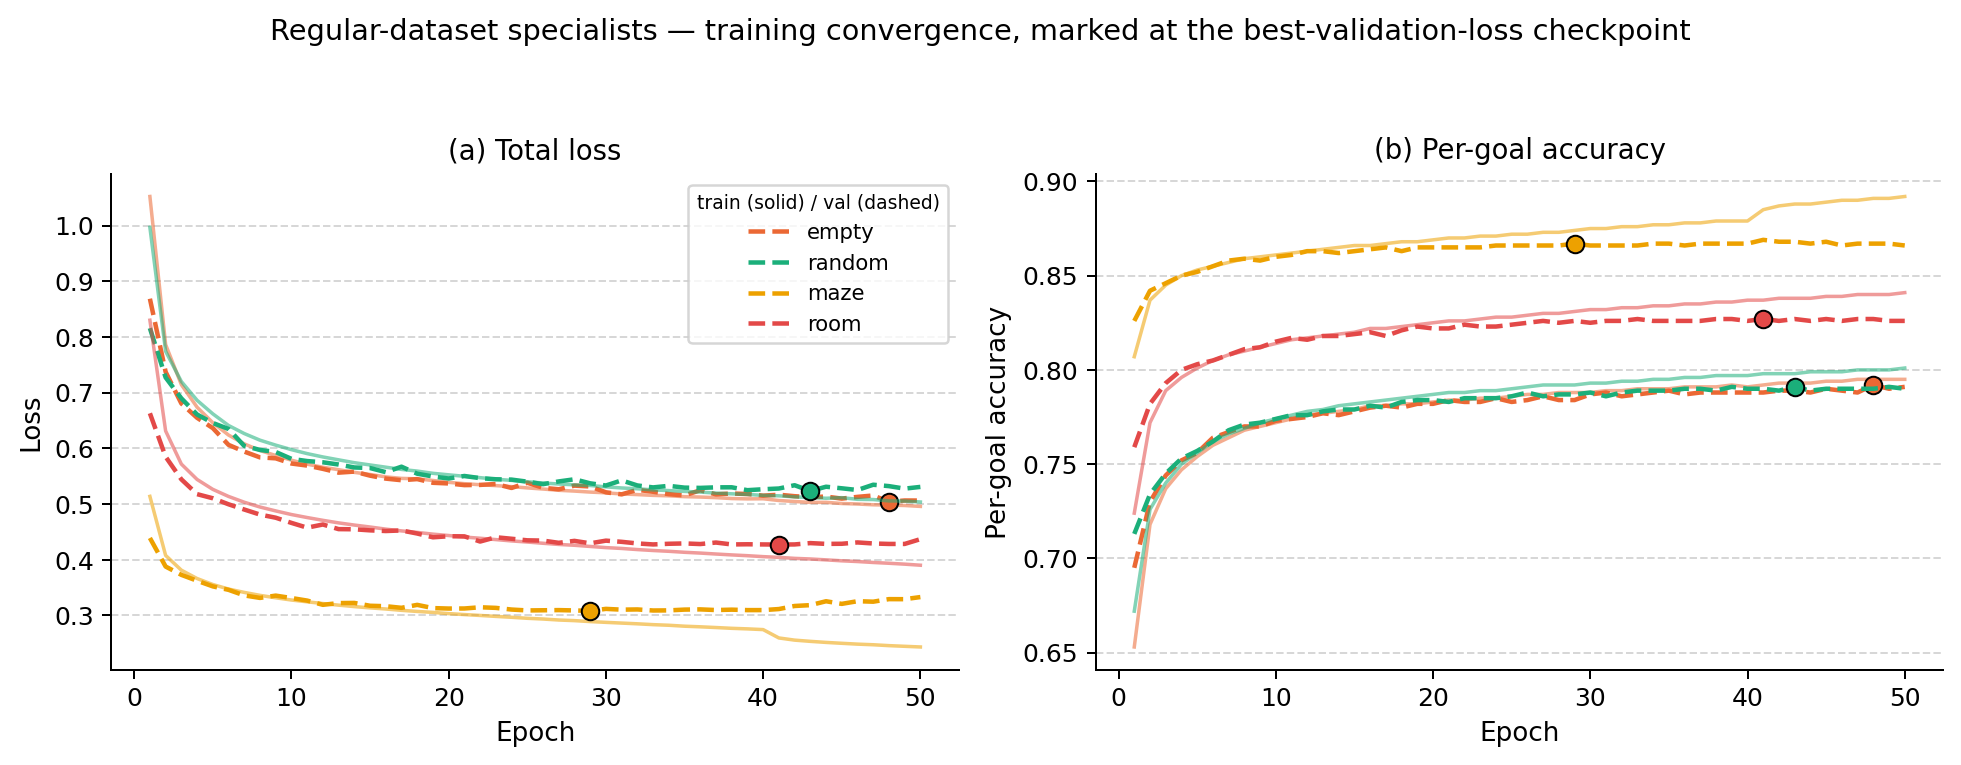
\includegraphics[width=0.92\textwidth]{fig_tierB_convergence.png}
\caption{Training convergence for the regular-dataset specialists — the only 4 of the 10
models whose per-epoch logs were pulled from the cluster. Circles mark the best-validation-loss
checkpoint. The signature is milder than the earlier large-model run (Section~\ref{sec:design}):
\texttt{empty} and \texttt{random} are still improving at the 50-epoch budget's end (best epoch
48 and 43), while \texttt{maze} and \texttt{room} peak earlier (epoch 29 and 41) and drift upward
afterward, so best-validation checkpointing still does some work but is not doing heavy lifting
here the way it did in Section~\ref{sec:design}. The large-dataset logs and the regular-dataset
generalist were not pulled for this report.}
\label{fig:tierBconv}
\end{figure}

\subsection*{Raw data}

Per-instance CSVs, aggregates and the model inventory live under \texttt{report/data/exp16/},
tracked in the repository (unlike \texttt{results/}, which is git-ignored). Per-instance columns:
\texttt{inst\_seed, cost\_nn, cost\_solver, nn\_k, solver\_k, conflicts\_nn, conflicts\_solver,
alloc\_ms, nn\_plan\_ms, solver\_ms}, written by \texttt{evaluation/full\_pipeline\_eval.py}.
\texttt{report/data/exp16/manifest.md} documents what is and is not included and the remaining
open items (offline accuracy, training logs in the requested per-epoch format, and cluster job
identifiers). The raw files and the manifest keep the original run names: \texttt{tierA\_*} holds
the large-dataset models and \texttt{tierB\_*} the regular-dataset ones. This report uses the
descriptive names throughout, and the model identifiers in Tables~\ref{tab:modelinv}
and~\ref{tab:modelinvB} are the literal directory names, so they can be matched to the files
directly.

\end{document}
